\documentclass[11pt]{article}
% Reproducible PDF bytes: no creation date, no random trailer identifier, no producer banner.
\pdfinfoomitdate=1
\pdftrailerid{}
\pdfsuppressptexinfo=-1

\usepackage[letterpaper,margin=1in]{geometry}
\usepackage[T1]{fontenc}
\usepackage{mathptmx}
\usepackage[scaled=0.92]{helvet}
\usepackage{microtype}
\usepackage{amsmath,amssymb,bm}
\usepackage{graphicx}
\usepackage{booktabs,tabularx,multirow,array,makecell,longtable}
\usepackage[font=small,labelfont=bf,skip=4pt]{caption}
\usepackage[dvipsnames]{xcolor}
\usepackage{enumitem}
\usepackage{float}
\usepackage[section]{placeins}
\usepackage{needspace}
\usepackage[numbers,sort&compress]{natbib}
\setlength{\bibsep}{1.5pt}
\renewcommand{\bibfont}{\small\raggedright}
\usepackage[hidelinks,pdftitle={First-order estimates find the influential cell types in the FlyVis models but misjudge their silencing effects: the nonlinearity is in the readout},pdfauthor={Richard Jeevash},pdfcreator={},pdfproducer={}]{hyperref}
\usepackage[nameinlink,capitalise]{cleveref}

\setlist{itemsep=2pt,topsep=3pt,parsep=0pt}
\setlength{\parskip}{3pt}
\renewcommand{\arraystretch}{1.12}
\newcolumntype{Y}{>{\raggedright\arraybackslash}X}
\crefname{appendix}{Appendix}{Appendices}
\renewcommand{\topfraction}{0.9}
\renewcommand{\bottomfraction}{0.8}
\renewcommand{\textfraction}{0.07}
\renewcommand{\floatpagefraction}{0.8}
\setcounter{topnumber}{3}
\setcounter{totalnumber}{5}

\newcommand{\DSI}{\mathrm{DSI}}
\newcommand{\relu}{\operatorname{relu}}
% Generated table bodies are read with the TeX primitive: LaTeX's \input runs file hooks, which inside a
% tabular would add an empty row.
\makeatletter\newcommand{\tableinput}[1]{\@@input #1 }\makeatother

% The macros of both studies (paper/make_numbers.py).
% Generated by paper/make_numbers.py: the union of the two studies' generated/numbers.tex. Do not edit.
% Study 1 = study-1-first-order, Study 2 = study-2-causes.
% Macros defined by both studies, with the same value: AmpLimit, LargeThreshold, NConfModels, NDevModels, NDirections, NModels.
\newcommand{\AbolishedByLOne}{79}
\newcommand{\AbolishedByMiFour}{45}
\newcommand{\AbolishedByMiOne}{152}
\newcommand{\AbolishedByTmThree}{39}
\newcommand{\AbolishedFull}{723}
\newcommand{\AbolishedFullPct}{1.6}
\newcommand{\AbolishedHalf}{254}
\newcommand{\AbolishedNoPreferred}{46}
\newcommand{\AbolishedSelectiveFull}{524}
\newcommand{\AbolishedSelectiveHalf}{178}
\newcommand{\AbolitionReadoutsFull}{275}
\newcommand{\AbsPredAboveOneFull}{722}
\newcommand{\AbsPredAboveOneHalf}{277}
\newcommand{\AmpLimit}{100}
\newcommand{\AmpLimitHigh}{1000}
\newcommand{\AmpLimitLow}{10}
\newcommand{\AmpRatioAboveTwoPct}{5.8}
\newcommand{\AmpRatioBelowHalfPct}{4.8}
\newcommand{\AmpRatioHighQ}{2.23}
\newcommand{\AmpRatioLargeDecMedian}{1.39}
\newcommand{\AmpRatioLargeIncMedian}{0.58}
\newcommand{\AmpRatioLargeMedian}{1.19}
\newcommand{\AmpRatioLargeQOne}{0.65}
\newcommand{\AmpRatioLargeQThree}{2.12}
\newcommand{\AmpRatioLowQ}{0.51}
\newcommand{\AmpRatioMedian}{1.00}
\newcommand{\AmpRatioQOne}{0.97}
\newcommand{\AmpRatioQThree}{1.04}
\newcommand{\AmplifiedCasesFull}{154}
\newcommand{\AmplifiedCasesHalf}{24}
\newcommand{\AmplifiedInterventionsFull}{21}
\newcommand{\AmplifiedInterventionsHalf}{3}
\newcommand{\AmplifiedSelectiveFull}{61}
\newcommand{\AmplifiedSelectiveHalf}{8}
\newcommand{\AnatABCFull}{0.454}
\newcommand{\AnatABCHalf}{0.270}
\newcommand{\AnatABFull}{0.454}
\newcommand{\AnatABHalf}{0.270}
\newcommand{\AnatACFull}{0.468}
\newcommand{\AnatACHalf}{0.272}
\newcommand{\AnatAFull}{0.468}
\newcommand{\AnatAHalf}{0.272}
\newcommand{\AnatBCFull}{0.620}
\newcommand{\AnatBCHalf}{0.485}
\newcommand{\AnatBFull}{0.620}
\newcommand{\AnatBHalf}{0.485}
\newcommand{\AnatCFull}{0.646}
\newcommand{\AnatCHalf}{0.507}
\newcommand{\AnatCfNetFull}{0.646}
\newcommand{\AnatCfNetHalf}{0.507}
\newcommand{\AnatCfReadFull}{0.646}
\newcommand{\AnatCfReadHalf}{0.507}
\newcommand{\AnatMisMeanFull}{0.468}
\newcommand{\AnatMisMeanHalf}{0.272}
\newcommand{\AnatMisZeroFull}{0.646}
\newcommand{\AnatMisZeroHalf}{0.507}
\newcommand{\AnatRefFull}{0.646}
\newcommand{\AnatRefHalf}{0.507}
\newcommand{\AnatSplitRatioFull}{0.646}
\newcommand{\AnatSplitRatioHalf}{0.507}
\newcommand{\AnatSplitRespFull}{0.646}
\newcommand{\AnatSplitRespHalf}{0.507}
\newcommand{\BackwardOverType}{8}
\newcommand{\BatchSize}{48}
\newcommand{\BelowOneA}{24}
\newcommand{\BelowOneB}{8}
\newcommand{\BelowOneCfRead}{45}
\newcommand{\BelowOneRef}{7}
\newcommand{\BelowOneSplitRatio}{45}
\newcommand{\BiasABCFull}{\ensuremath{+}0.731}
\newcommand{\BiasABCHalf}{\ensuremath{+}0.186}
\newcommand{\BiasABFull}{\ensuremath{+}0.022}
\newcommand{\BiasABHalf}{\ensuremath{+}0.008}
\newcommand{\BiasACFull}{\ensuremath{+}0.459}
\newcommand{\BiasACHalf}{\ensuremath{+}0.117}
\newcommand{\BiasAFull}{\ensuremath{+}0.022}
\newcommand{\BiasAHalf}{\ensuremath{+}0.008}
\newcommand{\BiasBCFull}{\ensuremath{+}1.131}
\newcommand{\BiasBCHalf}{\ensuremath{+}0.293}
\newcommand{\BiasBFull}{\ensuremath{-}0.002}
\newcommand{\BiasBHalf}{\ensuremath{+}0.006}
\newcommand{\BiasCFull}{\ensuremath{+}1.074}
\newcommand{\BiasCHalf}{\ensuremath{+}0.277}
\newcommand{\BiasCIABCFull}{[0.085, 2.007]}
\newcommand{\BiasCIABCHalf}{[0.024, 0.503]}
\newcommand{\BiasCIABFull}{[0.016, 0.028]}
\newcommand{\BiasCIABHalf}{[0.005, 0.011]}
\newcommand{\BiasCIACFull}{[0.071, 1.211]}
\newcommand{\BiasCIACHalf}{[0.020, 0.303]}
\newcommand{\BiasCIAFull}{[0.014, 0.029]}
\newcommand{\BiasCIAHalf}{[0.004, 0.011]}
\newcommand{\BiasCIBCFull}{[0.789, 1.555]}
\newcommand{\BiasCIBCHalf}{[0.209, 0.398]}
\newcommand{\BiasCIBFull}{[\ensuremath{-}0.014, 0.010]}
\newcommand{\BiasCIBHalf}{[0.000, 0.011]}
\newcommand{\BiasCICFull}{[0.533, 1.917]}
\newcommand{\BiasCICHalf}{[0.144, 0.483]}
\newcommand{\BiasCICfNetFull}{[\ensuremath{-}0.053, 0.017]}
\newcommand{\BiasCICfNetHalf}{[0.004, 0.021]}
\newcommand{\BiasCICfReadFull}{[\ensuremath{-}0.011, \ensuremath{-}0.003]}
\newcommand{\BiasCICfReadHalf}{[\ensuremath{-}0.010, \ensuremath{-}0.004]}
\newcommand{\BiasCIFull}{[\ensuremath{-}0.019, 0.011]}
\newcommand{\BiasCIHalf}{[\ensuremath{-}0.002, 0.012]}
\newcommand{\BiasCIMisMeanFull}{[\ensuremath{-}0.031, \ensuremath{-}0.008]}
\newcommand{\BiasCIMisMeanHalf}{[\ensuremath{-}0.019, \ensuremath{-}0.008]}
\newcommand{\BiasCIMisZeroFull}{[0.053, 0.074]}
\newcommand{\BiasCIMisZeroHalf}{[0.029, 0.043]}
\newcommand{\BiasCIRefFull}{[\ensuremath{-}0.019, 0.011]}
\newcommand{\BiasCIRefHalf}{[\ensuremath{-}0.002, 0.012]}
\newcommand{\BiasCISplitRatioFull}{[0.036, 0.048]}
\newcommand{\BiasCISplitRatioHalf}{[0.018, 0.026]}
\newcommand{\BiasCISplitRespFull}{[\ensuremath{-}1.443, \ensuremath{-}0.384]}
\newcommand{\BiasCISplitRespHalf}{[\ensuremath{-}0.530, \ensuremath{-}0.145]}
\newcommand{\BiasCfNetFull}{\ensuremath{-}0.014}
\newcommand{\BiasCfNetHalf}{\ensuremath{+}0.013}
\newcommand{\BiasCfReadFull}{\ensuremath{-}0.007}
\newcommand{\BiasCfReadHalf}{\ensuremath{-}0.007}
\newcommand{\BiasFull}{\ensuremath{-}0.002}
\newcommand{\BiasHalf}{0.006}
\newcommand{\BiasMaxFull}{0.073}
\newcommand{\BiasMaxHalf}{0.042}
\newcommand{\BiasMinFull}{\ensuremath{-}0.276}
\newcommand{\BiasMinHalf}{\ensuremath{-}0.119}
\newcommand{\BiasMisMeanFull}{\ensuremath{-}0.019}
\newcommand{\BiasMisMeanHalf}{\ensuremath{-}0.013}
\newcommand{\BiasMisZeroFull}{\ensuremath{+}0.063}
\newcommand{\BiasMisZeroHalf}{\ensuremath{+}0.035}
\newcommand{\BiasPositiveFull}{25}
\newcommand{\BiasPositiveHalf}{32}
\newcommand{\BiasRefFull}{\ensuremath{-}0.002}
\newcommand{\BiasRefHalf}{\ensuremath{+}0.006}
\newcommand{\BiasSplitRatioFull}{\ensuremath{+}0.042}
\newcommand{\BiasSplitRatioHalf}{\ensuremath{+}0.022}
\newcommand{\BiasSplitRespFull}{\ensuremath{-}0.842}
\newcommand{\BiasSplitRespHalf}{\ensuremath{-}0.310}
\newcommand{\BioCTOneTFiveDSI}{\ensuremath{-}0.07}
\newcommand{\BioCTOneTFiveRatio}{2.00}
\newcommand{\BioCTOneTFourDSI}{\ensuremath{-}0.27}
\newcommand{\BioCTOneTFourRatio}{1.81}
\newcommand{\BioMiFourTFourDSI}{\ensuremath{-}0.50}
\newcommand{\BioMiFourTFourRatio}{1.70}
\newcommand{\BioMiNineTFourDSI}{\ensuremath{-}0.44}
\newcommand{\BioMiNineTFourRatio}{3.23}
\newcommand{\BioMiOneTFourConditions}{16}
\newcommand{\BioMiOneTFourDefined}{2}
\newcommand{\BioTmThreeTFourRatio}{0.60}
\newcommand{\BootReps}{5,000}
\newcommand{\BootstrapReps}{5,000}
\newcommand{\BootstrapSeed}{20261007}
\newcommand{\Budget}{10}
\newcommand{\CPUThreads}{2}
\newcommand{\ChangeAFull}{\ensuremath{-}0.42}
\newcommand{\ChangeAHalf}{\ensuremath{-}0.29}
\newcommand{\ChangeBFull}{\ensuremath{+}0.01}
\newcommand{\ChangeBHalf}{\ensuremath{-}0.03}
\newcommand{\ChangeCFull}{\ensuremath{+}8.63}
\newcommand{\ChangeCHalf}{\ensuremath{+}2.86}
\newcommand{\ChangeCIAFull}{[\ensuremath{-}0.59, \ensuremath{-}0.25]}
\newcommand{\ChangeCIAHalf}{[\ensuremath{-}0.40, \ensuremath{-}0.18]}
\newcommand{\ChangeCIBFull}{[\ensuremath{-}0.14, 0.15]}
\newcommand{\ChangeCIBHalf}{[\ensuremath{-}0.12, 0.06]}
\newcommand{\ChangeCICFull}{[4.54, 14.69]}
\newcommand{\ChangeCICHalf}{[1.49, 4.89]}
\newcommand{\CheckedFilesConf}{12,144}
\newcommand{\CheckedFilesDev}{2,620}
\newcommand{\ClipABCFull}{1.06}
\newcommand{\ClipABCHalf}{0.78}
\newcommand{\ClipABFull}{0.82}
\newcommand{\ClipABHalf}{0.63}
\newcommand{\ClipACFull}{1.05}
\newcommand{\ClipACHalf}{0.74}
\newcommand{\ClipAFull}{0.84}
\newcommand{\ClipAHalf}{0.64}
\newcommand{\ClipBCFull}{1.34}
\newcommand{\ClipBCHalf}{1.18}
\newcommand{\ClipBFull}{0.79}
\newcommand{\ClipBHalf}{0.67}
\newcommand{\ClipBetterFull}{40}
\newcommand{\ClipBetterHalf}{43}
\newcommand{\ClipCFull}{1.30}
\newcommand{\ClipCHalf}{1.09}
\newcommand{\ClipCfNetFull}{0.68}
\newcommand{\ClipCfNetHalf}{0.58}
\newcommand{\ClipCfReadFull}{0.55}
\newcommand{\ClipCfReadHalf}{0.48}
\newcommand{\ClipDiffCIFull}{[\ensuremath{-}0.024, \ensuremath{-}0.015]}
\newcommand{\ClipDiffCIHalf}{[\ensuremath{-}0.022, \ensuremath{-}0.016]}
\newcommand{\ClipDiffFull}{\ensuremath{-}0.019}
\newcommand{\ClipDiffHalf}{\ensuremath{-}0.019}
\newcommand{\ClipMisMeanFull}{1.87}
\newcommand{\ClipMisMeanHalf}{2.18}
\newcommand{\ClipMisZeroFull}{1.02}
\newcommand{\ClipMisZeroHalf}{1.00}
\newcommand{\ClipRefFull}{0.82}
\newcommand{\ClipRefHalf}{0.72}
\newcommand{\ClipSplitRatioFull}{0.76}
\newcommand{\ClipSplitRatioHalf}{0.64}
\newcommand{\ClipSplitRespFull}{0.68}
\newcommand{\ClipSplitRespHalf}{0.69}
\newcommand{\ClusterDownMaeFO}{0.197}
\newcommand{\ClusterDownMaeZero}{0.104}
\newcommand{\ClusterDownModels}{5}
\newcommand{\ClusterDownPrec}{0.833}
\newcommand{\ClusterUpMaeFO}{0.129}
\newcommand{\ClusterUpMaeFOHalf}{0.057}
\newcommand{\ClusterUpMaeZero}{0.101}
\newcommand{\ClusterUpMaeZeroHalf}{0.062}
\newcommand{\ClusterUpModels}{29}
\newcommand{\ClusterUpPrec}{0.830}
\newcommand{\ClusterWeakMaeFO}{0.198}
\newcommand{\ClusterWeakMaeZero}{0.100}
\newcommand{\ClusterWeakModels}{12}
\newcommand{\ClusterWeakPrec}{0.770}
\newcommand{\CompositeFOFull}{0.837}
\newcommand{\ConfirmationDoneTime}{11:35}
\newcommand{\DSIThresholdsOther}{0, 0.1, 0.3}
\newcommand{\DecBiasAFull}{biased upwards}
\newcommand{\DecBiasAHalf}{biased upwards}
\newcommand{\DecBiasBFull}{no detectable bias}
\newcommand{\DecBiasBHalf}{no detectable bias}
\newcommand{\DecBiasCFull}{biased upwards}
\newcommand{\DecBiasCHalf}{biased upwards}
\newcommand{\DecChangeAFull}{improves on the reference}
\newcommand{\DecChangeAHalf}{improves on the reference}
\newcommand{\DecChangeBFull}{no detectable change}
\newcommand{\DecChangeBHalf}{no detectable change}
\newcommand{\DecChangeCFull}{worse than the reference}
\newcommand{\DecChangeCHalf}{worse than the reference}
\newcommand{\DecMechMMFull}{readout dominates}
\newcommand{\DecMechMMHalf}{readout dominates}
\newcommand{\DecMechMPFull}{readout dominates}
\newcommand{\DecMechMPHalf}{readout dominates}
\newcommand{\DecMechZMFull}{readout dominates}
\newcommand{\DecMechZMHalf}{readout dominates}
\newcommand{\DecMechZPFull}{readout dominates}
\newcommand{\DecMechZPHalf}{readout dominates}
\newcommand{\DecScreenAFull}{screen kept}
\newcommand{\DecScreenAHalf}{screen kept}
\newcommand{\DecScreenBFull}{screen kept}
\newcommand{\DecScreenBHalf}{screen kept}
\newcommand{\DecScreenCFull}{screen kept}
\newcommand{\DecScreenCHalf}{screen kept}
\newcommand{\DecSplitMMFull}{ratio dominates}
\newcommand{\DecSplitMMHalf}{ratio dominates}
\newcommand{\DecSplitMPFull}{ratio dominates}
\newcommand{\DecSplitMPHalf}{ratio dominates}
\newcommand{\DecSplitZMFull}{ratio dominates}
\newcommand{\DecSplitZMHalf}{ratio dominates}
\newcommand{\DecSplitZPFull}{ratio dominates}
\newcommand{\DecSplitZPHalf}{ratio dominates}
\newcommand{\DecWrongAFull}{more wrong signs}
\newcommand{\DecWrongAHalf}{no detectable change}
\newcommand{\DecWrongBFull}{fewer wrong signs}
\newcommand{\DecWrongBHalf}{fewer wrong signs}
\newcommand{\DecWrongCFull}{more wrong signs}
\newcommand{\DecWrongCHalf}{more wrong signs}
\newcommand{\DecZeroAFull}{not distinguishable from zero}
\newcommand{\DecZeroAHalf}{beats zero}
\newcommand{\DecZeroBFull}{worse than zero}
\newcommand{\DecZeroBHalf}{not distinguishable from zero}
\newcommand{\DecZeroCFull}{worse than zero}
\newcommand{\DecZeroCHalf}{worse than zero}
\newcommand{\DenomThreshold}{\ensuremath{10^{-8}}}
\newcommand{\DevAFull}{1.09}
\newcommand{\DevAHalf}{0.73}
\newcommand{\DevAPointOne}{0.31}
\newcommand{\DevAQuarter}{0.50}
\newcommand{\DevAThreeQ}{0.93}
\newcommand{\DevBFull}{1.84}
\newcommand{\DevBHalf}{1.20}
\newcommand{\DevBPointOne}{0.51}
\newcommand{\DevBQuarter}{0.83}
\newcommand{\DevBThreeQ}{1.58}
\newcommand{\DevBetterFull}{0}
\newcommand{\DevBetterHalf}{3}
\newcommand{\DevBetterMaxStrength}{0.25}
\newcommand{\DevBetterOneTenth}{4}
\newcommand{\DevBetterQuarter}{3}
\newcommand{\DevBetterThreeQuarter}{0}
\newcommand{\DevCFull}{11.65}
\newcommand{\DevCHalf}{4.21}
\newcommand{\DevCPointOne}{0.90}
\newcommand{\DevCQuarter}{2.03}
\newcommand{\DevCThreeQ}{7.68}
\newcommand{\DevCfReadFull}{0.49}
\newcommand{\DevCfReadHalf}{0.38}
\newcommand{\DevCfReadPointOne}{0.31}
\newcommand{\DevCfReadQuarter}{0.35}
\newcommand{\DevCfReadThreeQ}{0.47}
\newcommand{\DevMaeClipFull}{0.094}
\newcommand{\DevMaeClipHalf}{0.054}
\newcommand{\DevMaeClipOneTenth}{0.010}
\newcommand{\DevMaeClipQuarter}{0.029}
\newcommand{\DevMaeClipThreeQuarter}{0.076}
\newcommand{\DevMaeFOFull}{0.174}
\newcommand{\DevMaeFOHalf}{0.079}
\newcommand{\DevMaeFOOneTenth}{0.011}
\newcommand{\DevMaeFOQuarter}{0.036}
\newcommand{\DevMaeFOThreeQuarter}{0.126}
\newcommand{\DevMaeZeroFull}{0.105}
\newcommand{\DevMaeZeroHalf}{0.068}
\newcommand{\DevMaeZeroOneTenth}{0.017}
\newcommand{\DevMaeZeroQuarter}{0.040}
\newcommand{\DevMaeZeroThreeQuarter}{0.088}
\newcommand{\DevModelList}{000, 001, 004 and 005}
\newcommand{\DevPrecAnatFull}{0.642}
\newcommand{\DevPrecAnatHalf}{0.522}
\newcommand{\DevPrecAnatOneTenth}{0.119}
\newcommand{\DevPrecAnatQuarter}{0.295}
\newcommand{\DevPrecAnatThreeQuarter}{0.599}
\newcommand{\DevPrecFOFull}{0.820}
\newcommand{\DevPrecFOHalf}{0.754}
\newcommand{\DevPrecFOOneTenth}{0.222}
\newcommand{\DevPrecFOQuarter}{0.556}
\newcommand{\DevPrecFOThreeQuarter}{0.791}
\newcommand{\DevRefFull}{1.56}
\newcommand{\DevRefHalf}{1.07}
\newcommand{\DevRefPointOne}{0.57}
\newcommand{\DevRefQuarter}{0.81}
\newcommand{\DevRefThreeQ}{1.33}
\newcommand{\DevSplitRatioFull}{0.68}
\newcommand{\DevSplitRatioHalf}{0.57}
\newcommand{\DevSplitRatioPointOne}{0.39}
\newcommand{\DevSplitRatioQuarter}{0.50}
\newcommand{\DevSplitRatioThreeQ}{0.65}
\newcommand{\DominanceFull}{(a) dominates}
\newcommand{\DominanceHalf}{(a) dominates}
\newcommand{\DsiRecomputeMaxErr}{\ensuremath{2.3\times 10^{-7}}}
\newcommand{\EdgesFlyVis}{1,513,231}
\newcommand{\ExactTieReadouts}{3}
\newcommand{\ExhaustivePerSec}{0.0069}
\newcommand{\ExtraStrengths}{0.1, 0.25, 0.75}
\newcommand{\FlagBudgetPrimary}{10}
\newcommand{\FlagPaysFiveClip}{no}
\newcommand{\FlagPaysFiveZero}{no}
\newcommand{\FlagPaysTenClip}{no}
\newcommand{\FlagPaysTenZero}{no}
\newcommand{\FlagPaysTwentyClip}{no}
\newcommand{\FlagPaysTwentyZero}{no}
\newcommand{\FlagPerSecFiveClip}{0.0021}
\newcommand{\FlagPerSecFiveZero}{0.0015}
\newcommand{\FlagPerSecTenClip}{0.0029}
\newcommand{\FlagPerSecTenZero}{0.0024}
\newcommand{\FlagPerSecTwentyClip}{0.0039}
\newcommand{\FlagPerSecTwentyZero}{0.0036}
\newcommand{\FlagRecFiveClip}{35}
\newcommand{\FlagRecFiveZero}{25}
\newcommand{\FlagRecTenClip}{53}
\newcommand{\FlagRecTenZero}{44}
\newcommand{\FlagRecTwentyClip}{79}
\newcommand{\FlagRecTwentyZero}{73}
\newcommand{\FlagSecFiveClip}{170}
\newcommand{\FlagSecFiveZero}{170}
\newcommand{\FlagSecTenClip}{181}
\newcommand{\FlagSecTenZero}{181}
\newcommand{\FlagSecTwentyClip}{204}
\newcommand{\FlagSecTwentyZero}{204}
\newcommand{\FramesFast}{86}
\newcommand{\FramesSlow}{344}
\newcommand{\FreezeAISixInputs}{8}
\newcommand{\FreezeFiles}{20}
\newcommand{\FreezeTime}{04:48}
\newcommand{\FreezeTwoFiles}{24}
\newcommand{\FreezeTwoRecordModels}{15}
\newcommand{\FrozenFiles}{182}
\newcommand{\GateAbsTmThreeMax}{\ensuremath{1.8\times 10^{-4}}}
\newcommand{\GateAbsTmThreeModel}{039}
\newcommand{\GateNormMax}{\ensuremath{1.0\times 10^{-6}}}
\newcommand{\InclAnatCIFull}{[0.339, 0.393]}
\newcommand{\InclAnatCIHalf}{[0.238, 0.285]}
\newcommand{\InclAnatFourFull}{0.370}
\newcommand{\InclAnatFourHalf}{0.271}
\newcommand{\InclAnatFull}{0.367}
\newcommand{\InclAnatHalf}{0.262}
\newcommand{\InclCurrentFull}{0.311}
\newcommand{\InclCurrentHalf}{0.218}
\newcommand{\InclDiffAnatCIFull}{[0.066, 0.099]}
\newcommand{\InclDiffAnatCIHalf}{[0.099, 0.131]}
\newcommand{\InclDiffAnatFull}{0.082}
\newcommand{\InclDiffAnatHalf}{0.115}
\newcommand{\InclDirectFull}{0.302}
\newcommand{\InclDirectHalf}{0.209}
\newcommand{\InclFOCIFull}{[0.417, 0.481]}
\newcommand{\InclFOCIHalf}{[0.347, 0.404]}
\newcommand{\InclFOFull}{0.449}
\newcommand{\InclFOHalf}{0.376}
\newcommand{\InclLossesAnatFull}{2}
\newcommand{\InclLossesAnatHalf}{0}
\newcommand{\InclMaeClipFull}{0.049}
\newcommand{\InclMaeFOFull}{0.091}
\newcommand{\InclMaeZeroFull}{0.055}
\newcommand{\InclRandomFull}{0.159}
\newcommand{\InclRandomHalf}{0.103}
\newcommand{\InclRandomLowDSIFull}{0.044}
\newcommand{\InclRandomLowDSIHalf}{0.023}
\newcommand{\InclRandomMainDSIFull}{0.296}
\newcommand{\InclRandomMainDSIHalf}{0.199}
\newcommand{\InclReadoutsFull}{697}
\newcommand{\InclReadoutsHalf}{697}
\newcommand{\InclTiesAnatFull}{2}
\newcommand{\InclTiesAnatHalf}{0}
\newcommand{\InclTrainedFull}{0.330}
\newcommand{\InclTrainedHalf}{0.230}
\newcommand{\InclWinsAnatFull}{42}
\newcommand{\InclWinsAnatHalf}{46}
\newcommand{\IndexedTypePairs}{604}
\newcommand{\InputDirectCases}{3,027}
\newcommand{\InputIndirectCases}{16,798}
\newcommand{\InteractionCIMMFull}{[0.68, 2.15]}
\newcommand{\InteractionCIMMHalf}{[0.47, 1.28]}
\newcommand{\InteractionCIMPFull}{[0.31, 1.00]}
\newcommand{\InteractionCIMPHalf}{[0.17, 0.58]}
\newcommand{\InteractionCIZMFull}{[7.29, 51.66]}
\newcommand{\InteractionCIZMHalf}{[5.41, 38.16]}
\newcommand{\InteractionCIZPFull}{[1.75, 7.78]}
\newcommand{\InteractionCIZPHalf}{[1.36, 6.31]}
\newcommand{\InteractionMMFull}{1.33}
\newcommand{\InteractionMMHalf}{0.82}
\newcommand{\InteractionMPFull}{0.61}
\newcommand{\InteractionMPHalf}{0.35}
\newcommand{\InteractionZMFull}{25.05}
\newcommand{\InteractionZMHalf}{18.24}
\newcommand{\InteractionZPFull}{4.33}
\newcommand{\InteractionZPHalf}{3.46}
\newcommand{\LargeDecFull}{4,419}
\newcommand{\LargeDecPredIncPct}{23.6}
\newcommand{\LargeDecreasePct}{80}
\newcommand{\LargeFull}{5,501}
\newcommand{\LargeFullPct}{27.7}
\newcommand{\LargeHalf}{3,890}
\newcommand{\LargeIncFull}{1,082}
\newcommand{\LargeIncPredDecPct}{13.8}
\newcommand{\LargeThreshold}{0.1}
\newcommand{\LowDSI}{383}
\newcommand{\LowDSICasesFull}{24,696}
\newcommand{\LowerThanRefA}{41}
\newcommand{\LowerThanRefB}{25}
\newcommand{\LowerThanRefCfRead}{45}
\newcommand{\LowerThanRefSplitRatio}{44}
\newcommand{\MaeABCFull}{0.748}
\newcommand{\MaeABCHalf}{0.190}
\newcommand{\MaeABFull}{0.061}
\newcommand{\MaeABHalf}{0.024}
\newcommand{\MaeACFull}{0.477}
\newcommand{\MaeACHalf}{0.123}
\newcommand{\MaeAFull}{0.060}
\newcommand{\MaeAHalf}{0.024}
\newcommand{\MaeBCFull}{1.327}
\newcommand{\MaeBCHalf}{0.344}
\newcommand{\MaeBFull}{0.160}
\newcommand{\MaeBHalf}{0.071}
\newcommand{\MaeBetterFull}{7}
\newcommand{\MaeBetterHalf}{28}
\newcommand{\MaeCFull}{1.173}
\newcommand{\MaeCHalf}{0.304}
\newcommand{\MaeCfNetFull}{0.184}
\newcommand{\MaeCfNetHalf}{0.060}
\newcommand{\MaeCfReadFull}{0.054}
\newcommand{\MaeCfReadHalf}{0.030}
\newcommand{\MaeClipFull}{0.082}
\newcommand{\MaeClipHalf}{0.046}
\newcommand{\MaeDiffABCFull}{\ensuremath{+}0.695}
\newcommand{\MaeDiffABCHalf}{\ensuremath{+}0.161}
\newcommand{\MaeDiffABFull}{\ensuremath{+}0.008}
\newcommand{\MaeDiffABHalf}{\ensuremath{-}0.005}
\newcommand{\MaeDiffACFull}{\ensuremath{+}0.425}
\newcommand{\MaeDiffACHalf}{\ensuremath{+}0.094}
\newcommand{\MaeDiffAFull}{\ensuremath{+}0.008}
\newcommand{\MaeDiffAHalf}{\ensuremath{-}0.005}
\newcommand{\MaeDiffBCFull}{\ensuremath{+}1.223}
\newcommand{\MaeDiffBCHalf}{\ensuremath{+}0.276}
\newcommand{\MaeDiffBFull}{\ensuremath{+}0.056}
\newcommand{\MaeDiffBHalf}{\ensuremath{+}0.004}
\newcommand{\MaeDiffCFull}{\ensuremath{+}1.072}
\newcommand{\MaeDiffCHalf}{\ensuremath{+}0.239}
\newcommand{\MaeDiffCIABCFull}{[0.049, 1.968]}
\newcommand{\MaeDiffCIABCHalf}{[0.002, 0.476]}
\newcommand{\MaeDiffCIABFull}{[\ensuremath{-}0.001, 0.022]}
\newcommand{\MaeDiffCIABHalf}{[\ensuremath{-}0.009, 0.001]}
\newcommand{\MaeDiffCIACFull}{[0.038, 1.174]}
\newcommand{\MaeDiffCIACHalf}{[\ensuremath{-}0.001, 0.278]}
\newcommand{\MaeDiffCIAFull}{[\ensuremath{-}0.0003, 0.0199]}
\newcommand{\MaeDiffCIAHalf}{[\ensuremath{-}0.0082, \ensuremath{-}0.0001]}
\newcommand{\MaeDiffCIBCFull}{[0.820, 1.710]}
\newcommand{\MaeDiffCIBCHalf}{[0.180, 0.393]}
\newcommand{\MaeDiffCIBFull}{[0.034, 0.084]}
\newcommand{\MaeDiffCIBHalf}{[\ensuremath{-}0.005, 0.015]}
\newcommand{\MaeDiffCICFull}{[0.523, 1.904]}
\newcommand{\MaeDiffCICHalf}{[0.106, 0.440]}
\newcommand{\MaeDiffCICfNetFull}{[0.052, 0.119]}
\newcommand{\MaeDiffCICfNetHalf}{[\ensuremath{-}0.011, 0.002]}
\newcommand{\MaeDiffCICfReadFull}{[\ensuremath{-}0.054, \ensuremath{-}0.041]}
\newcommand{\MaeDiffCICfReadHalf}{[\ensuremath{-}0.040, \ensuremath{-}0.030]}
\newcommand{\MaeDiffCIFull}{[0.034, 0.074]}
\newcommand{\MaeDiffCIHalf}{[\ensuremath{-}0.003, 0.013]}
\newcommand{\MaeDiffCIMisMeanFull}{[0.099, 0.158]}
\newcommand{\MaeDiffCIMisMeanHalf}{[0.046, 0.075]}
\newcommand{\MaeDiffCIMisZeroFull}{[0.009, 0.037]}
\newcommand{\MaeDiffCIMisZeroHalf}{[0.0005, 0.0138]}
\newcommand{\MaeDiffCIRefFull}{[0.035, 0.075]}
\newcommand{\MaeDiffCIRefHalf}{[\ensuremath{-}0.002, 0.013]}
\newcommand{\MaeDiffCISplitRatioFull}{[\ensuremath{-}0.030, \ensuremath{-}0.021]}
\newcommand{\MaeDiffCISplitRatioHalf}{[\ensuremath{-}0.028, \ensuremath{-}0.020]}
\newcommand{\MaeDiffCISplitRespFull}{[0.326, 1.380]}
\newcommand{\MaeDiffCISplitRespHalf}{[0.102, 0.483]}
\newcommand{\MaeDiffCfNetFull}{\ensuremath{+}0.083}
\newcommand{\MaeDiffCfNetHalf}{\ensuremath{-}0.005}
\newcommand{\MaeDiffCfReadFull}{\ensuremath{-}0.047}
\newcommand{\MaeDiffCfReadHalf}{\ensuremath{-}0.035}
\newcommand{\MaeDiffFull}{0.054}
\newcommand{\MaeDiffHalf}{0.005}
\newcommand{\MaeDiffMisMeanFull}{\ensuremath{+}0.127}
\newcommand{\MaeDiffMisMeanHalf}{\ensuremath{+}0.060}
\newcommand{\MaeDiffMisZeroFull}{\ensuremath{+}0.021}
\newcommand{\MaeDiffMisZeroHalf}{\ensuremath{+}0.006}
\newcommand{\MaeDiffRefFull}{\ensuremath{+}0.054}
\newcommand{\MaeDiffRefHalf}{\ensuremath{+}0.005}
\newcommand{\MaeDiffSplitRatioFull}{\ensuremath{-}0.025}
\newcommand{\MaeDiffSplitRatioHalf}{\ensuremath{-}0.024}
\newcommand{\MaeDiffSplitRespFull}{\ensuremath{+}0.781}
\newcommand{\MaeDiffSplitRespHalf}{\ensuremath{+}0.266}
\newcommand{\MaeDirectFull}{0.331}
\newcommand{\MaeFOCIFull}{[0.132, 0.179]}
\newcommand{\MaeFOCIHalf}{[0.059, 0.082]}
\newcommand{\MaeFOFull}{0.155}
\newcommand{\MaeFOHalf}{0.070}
\newcommand{\MaeIndirectFull}{0.122}
\newcommand{\MaeLargeFOFull}{0.466}
\newcommand{\MaeLargeFOHalf}{0.277}
\newcommand{\MaeLargeWorseFull}{37}
\newcommand{\MaeLargeWorseHalf}{17}
\newcommand{\MaeLargeZeroFull}{0.316}
\newcommand{\MaeLargeZeroHalf}{0.263}
\newcommand{\MaeLowDSIFull}{0.035}
\newcommand{\MaeMisMeanFull}{0.180}
\newcommand{\MaeMisMeanHalf}{0.088}
\newcommand{\MaeMisZeroFull}{0.122}
\newcommand{\MaeMisZeroHalf}{0.071}
\newcommand{\MaeRefFull}{0.155}
\newcommand{\MaeRefHalf}{0.070}
\newcommand{\MaeSplitRatioFull}{0.075}
\newcommand{\MaeSplitRatioHalf}{0.041}
\newcommand{\MaeSplitRespFull}{0.882}
\newcommand{\MaeSplitRespHalf}{0.331}
\newcommand{\MaeWorseFull}{39}
\newcommand{\MaeWorseHalf}{18}
\newcommand{\MaeZeroABCFull}{0.053}
\newcommand{\MaeZeroABCHalf}{0.029}
\newcommand{\MaeZeroABFull}{0.053}
\newcommand{\MaeZeroABHalf}{0.029}
\newcommand{\MaeZeroACFull}{0.053}
\newcommand{\MaeZeroACHalf}{0.029}
\newcommand{\MaeZeroAFull}{0.053}
\newcommand{\MaeZeroAHalf}{0.029}
\newcommand{\MaeZeroBCFull}{0.104}
\newcommand{\MaeZeroBCHalf}{0.067}
\newcommand{\MaeZeroBFull}{0.104}
\newcommand{\MaeZeroBHalf}{0.067}
\newcommand{\MaeZeroCFull}{0.101}
\newcommand{\MaeZeroCHalf}{0.065}
\newcommand{\MaeZeroCIFull}{[0.093, 0.109]}
\newcommand{\MaeZeroCIHalf}{[0.059, 0.071]}
\newcommand{\MaeZeroCfNetFull}{0.101}
\newcommand{\MaeZeroCfNetHalf}{0.065}
\newcommand{\MaeZeroCfReadFull}{0.101}
\newcommand{\MaeZeroCfReadHalf}{0.065}
\newcommand{\MaeZeroFull}{0.101}
\newcommand{\MaeZeroHalf}{0.065}
\newcommand{\MaeZeroLowDSIFull}{0.017}
\newcommand{\MaeZeroMisMeanFull}{0.053}
\newcommand{\MaeZeroMisMeanHalf}{0.029}
\newcommand{\MaeZeroMisZeroFull}{0.101}
\newcommand{\MaeZeroMisZeroHalf}{0.065}
\newcommand{\MaeZeroPeakChangedFull}{0.378}
\newcommand{\MaeZeroPeakSameFull}{0.088}
\newcommand{\MaeZeroRefFull}{0.101}
\newcommand{\MaeZeroRefHalf}{0.065}
\newcommand{\MaeZeroSplitRatioFull}{0.101}
\newcommand{\MaeZeroSplitRatioHalf}{0.065}
\newcommand{\MaeZeroSplitRespFull}{0.101}
\newcommand{\MaeZeroSplitRespHalf}{0.065}
\newcommand{\MainCasesFull}{19,825}
\newcommand{\MainCasesHalf}{20,224}
\newcommand{\MainDSI}{0.2}
\newcommand{\MainReadouts}{314}
\newcommand{\MaxAbsPredFull}{17.4}
\newcommand{\MaxAbsPredHalf}{8.7}
\newcommand{\MedianErrLargeFull}{0.243}
\newcommand{\MedianErrSmallFull}{0.002}
\newcommand{\MisMeanMinusMatchedCIFull}{[1.82, 2.60]}
\newcommand{\MisMeanMinusMatchedCIHalf}{[1.88, 2.57]}
\newcommand{\MisMeanMinusMatchedFull}{\ensuremath{+}2.21}
\newcommand{\MisMeanMinusMatchedHalf}{\ensuremath{+}2.22}
\newcommand{\MisMeanTopAnatCIFull}{[\ensuremath{-}0.022, 0.025]}
\newcommand{\MisMeanTopAnatCIHalf}{[0.025, 0.058]}
\newcommand{\MisMeanTopAnatFull}{\ensuremath{+}0.001}
\newcommand{\MisMeanTopAnatHalf}{\ensuremath{+}0.041}
\newcommand{\MisZeroMinusRefCIFull}{[\ensuremath{-}0.45, \ensuremath{-}0.14]}
\newcommand{\MisZeroMinusRefCIHalf}{[\ensuremath{-}0.05, 0.15]}
\newcommand{\MisZeroMinusRefFull}{\ensuremath{-}0.29}
\newcommand{\MisZeroMinusRefHalf}{\ensuremath{+}0.05}
\newcommand{\NCasesFull}{19,825}
\newcommand{\NConfModels}{46}
\newcommand{\NDevModels}{4}
\newcommand{\NDirections}{12}
\newcommand{\NLargeFull}{5,501}
\newcommand{\NModels}{50}
\newcommand{\NReadoutTypes}{8}
\newcommand{\NReadouts}{8}
\newcommand{\NSimTypes}{63}
\newcommand{\NTrajectories}{24}
\newcommand{\NTypes}{65}
\newcommand{\NUnitsAll}{736}
\newcommand{\NUnitsEligible}{314}
\newcommand{\NearTieReadouts}{45}
\newcommand{\NetEdges}{1,513,231}
\newcommand{\NetNodes}{45,669}
\newcommand{\NetTypePairs}{604}
\newcommand{\NetTypes}{65}
\newcommand{\NodesFlyVis}{45,669}
\newcommand{\OriginalFiles}{3,228}
\newcommand{\OutsideFull}{8.7}
\newcommand{\OutsideHalf}{4.4}
\newcommand{\PairMiOneMiFourDSI}{0.584}
\newcommand{\PairTmCount}{4}
\newcommand{\PairTmMaxDSI}{0.020}
\newcommand{\PairTmSubadditiveMajority}{3}
\newcommand{\PearsonPooledFull}{0.35}
\newcommand{\PearsonPooledHalf}{0.46}
\newcommand{\PilotAutoKMax}{1.1}
\newcommand{\PilotAutodiffMax}{\ensuremath{5.9\times 10^{-8}}}
\newcommand{\PilotFDJMax}{\ensuremath{1.0\times 10^{-4}}}
\newcommand{\PilotFDKMax}{201}
\newcommand{\PilotFDKMin}{100}
\newcommand{\PilotGradMax}{\ensuremath{2.5\times 10^{-6}}}
\newcommand{\PostCases}{19,825}
\newcommand{\PostLargeDenFrac}{12}
\newcommand{\PostLargeDenShare}{86}
\newcommand{\PostLargeFirst}{0.76}
\newcommand{\PostLargeSecond}{7.8}
\newcommand{\PostLargeZero}{0.34}
\newcommand{\PostRestFirst}{0.066}
\newcommand{\PostRestSecond}{0.082}
\newcommand{\PostRestSecondBelowFirst}{0}
\newcommand{\PostRestZero}{0.068}
\newcommand{\PostSecondErrLarge}{7.85}
\newcommand{\PostSecondErrRest}{0.082}
\newcommand{\PostShareReadout}{78}
\newcommand{\PostWrongFirst}{21.7}
\newcommand{\PostWrongRead}{9.1}
\newcommand{\PrecAnatCIFull}{[0.620, 0.673]}
\newcommand{\PrecAnatCIHalf}{[0.477, 0.539]}
\newcommand{\PrecAnatFourFull}{0.672}
\newcommand{\PrecAnatFourHalf}{0.532}
\newcommand{\PrecAnatFull}{0.646}
\newcommand{\PrecAnatHalf}{0.507}
\newcommand{\PrecAnatOneFull}{0.522}
\newcommand{\PrecAnatOneHalf}{0.411}
\newcommand{\PrecAnatTwoFull}{0.634}
\newcommand{\PrecAnatTwoHalf}{0.497}
\newcommand{\PrecCurrentFull}{0.539}
\newcommand{\PrecCurrentHalf}{0.432}
\newcommand{\PrecDiffAnatCIFull}{[0.140, 0.199]}
\newcommand{\PrecDiffAnatCIHalf}{[0.188, 0.243]}
\newcommand{\PrecDiffAnatFourCIFull}{[0.116, 0.172]}
\newcommand{\PrecDiffAnatFourFull}{0.143}
\newcommand{\PrecDiffAnatFull}{0.169}
\newcommand{\PrecDiffAnatHalf}{0.214}
\newcommand{\PrecDirectFull}{0.522}
\newcommand{\PrecDirectHalf}{0.411}
\newcommand{\PrecDistFull}{0.520}
\newcommand{\PrecDistHalf}{0.408}
\newcommand{\PrecFOCIFull}{[0.784, 0.845]}
\newcommand{\PrecFOCIHalf}{[0.685, 0.757]}
\newcommand{\PrecFOFull}{0.815}
\newcommand{\PrecFOHalf}{0.722}
\newcommand{\PrecLossesAnatFull}{2}
\newcommand{\PrecLossesAnatHalf}{0}
\newcommand{\PrecRandomFull}{0.277}
\newcommand{\PrecRandomHalf}{0.193}
\newcommand{\PrecTiesAnatFull}{1}
\newcommand{\PrecTiesAnatHalf}{0}
\newcommand{\PrecTrainedFull}{0.592}
\newcommand{\PrecTrainedHalf}{0.456}
\newcommand{\PrecWinsAnatFourFull}{43}
\newcommand{\PrecWinsAnatFull}{43}
\newcommand{\PrecWinsAnatHalf}{46}
\newcommand{\PredAddendumHeld}{28}
\newcommand{\PredAddendumTotal}{29}
\newcommand{\PredPrimaryHeld}{22}
\newcommand{\PredPrimaryTotal}{27}
\newcommand{\RatioABCFull}{9.62}
\newcommand{\RatioABCHalf}{3.81}
\newcommand{\RatioABFull}{1.09}
\newcommand{\RatioABHalf}{0.75}
\newcommand{\RatioACFull}{6.70}
\newcommand{\RatioACHalf}{2.71}
\newcommand{\RatioAFull}{1.09}
\newcommand{\RatioAHalf}{0.76}
\newcommand{\RatioBCFull}{11.60}
\newcommand{\RatioBCHalf}{4.50}
\newcommand{\RatioBFull}{1.52}
\newcommand{\RatioBHalf}{1.02}
\newcommand{\RatioCFull}{10.14}
\newcommand{\RatioCHalf}{3.91}
\newcommand{\RatioCIABCFull}{[1.88, 24.79]}
\newcommand{\RatioCIABCHalf}{[0.99, 9.33]}
\newcommand{\RatioCIABFull}{[0.96, 1.26]}
\newcommand{\RatioCIABHalf}{[0.66, 0.88]}
\newcommand{\RatioCIACFull}{[1.66, 16.34]}
\newcommand{\RatioCIACHalf}{[0.88, 6.23]}
\newcommand{\RatioCIAFull}{[0.97, 1.26]}
\newcommand{\RatioCIAHalf}{[0.67, 0.87]}
\newcommand{\RatioCIBCFull}{[8.66, 15.02]}
\newcommand{\RatioCIBCHalf}{[3.50, 5.64]}
\newcommand{\RatioCIBFull}{[1.34, 1.73]}
\newcommand{\RatioCIBHalf}{[0.92, 1.14]}
\newcommand{\RatioCICFull}{[5.93, 16.34]}
\newcommand{\RatioCICHalf}{[2.47, 5.99]}
\newcommand{\RatioCICfNetFull}{[1.50, 2.09]}
\newcommand{\RatioCICfNetHalf}{[0.79, 0.99]}
\newcommand{\RatioCICfReadFull}{[0.51, 0.60]}
\newcommand{\RatioCICfReadHalf}{[0.44, 0.53]}
\newcommand{\RatioCIMisMeanFull}{[2.92, 3.71]}
\newcommand{\RatioCIMisMeanHalf}{[2.64, 3.32]}
\newcommand{\RatioCIMisZeroFull}{[1.09, 1.38]}
\newcommand{\RatioCIMisZeroHalf}{[1.00, 1.21]}
\newcommand{\RatioCIRefFull}{[1.34, 1.71]}
\newcommand{\RatioCIRefHalf}{[0.94, 1.16]}
\newcommand{\RatioCISplitRatioFull}{[0.73, 0.80]}
\newcommand{\RatioCISplitRatioHalf}{[0.60, 0.69]}
\newcommand{\RatioCISplitRespFull}{[3.81, 12.02]}
\newcommand{\RatioCISplitRespHalf}{[2.30, 6.74]}
\newcommand{\RatioCfNetFull}{1.78}
\newcommand{\RatioCfNetHalf}{0.88}
\newcommand{\RatioCfReadFull}{0.55}
\newcommand{\RatioCfReadHalf}{0.48}
\newcommand{\RatioMinusRespCIMMFull}{[0.83, 2.28]}
\newcommand{\RatioMinusRespCIMMHalf}{[0.32, 1.13]}
\newcommand{\RatioMinusRespCIMPFull}{[0.44, 1.16]}
\newcommand{\RatioMinusRespCIMPHalf}{[0.18, 0.62]}
\newcommand{\RatioMinusRespCIZMFull}{[7.44, 51.84]}
\newcommand{\RatioMinusRespCIZMHalf}{[5.32, 38.05]}
\newcommand{\RatioMinusRespCIZPFull}{[2.05, 8.05]}
\newcommand{\RatioMinusRespCIZPHalf}{[1.55, 6.46]}
\newcommand{\RatioMinusRespMMFull}{1.46}
\newcommand{\RatioMinusRespMMHalf}{0.67}
\newcommand{\RatioMinusRespMPFull}{0.76}
\newcommand{\RatioMinusRespMPHalf}{0.38}
\newcommand{\RatioMinusRespZMFull}{25.19}
\newcommand{\RatioMinusRespZMHalf}{18.14}
\newcommand{\RatioMinusRespZPFull}{4.61}
\newcommand{\RatioMinusRespZPHalf}{3.62}
\newcommand{\RatioMisMeanFull}{3.30}
\newcommand{\RatioMisMeanHalf}{2.98}
\newcommand{\RatioMisZeroFull}{1.22}
\newcommand{\RatioMisZeroHalf}{1.09}
\newcommand{\RatioRefFull}{1.51}
\newcommand{\RatioRefHalf}{1.05}
\newcommand{\RatioSplitRatioFull}{0.76}
\newcommand{\RatioSplitRatioHalf}{0.64}
\newcommand{\RatioSplitRespFull}{7.39}
\newcommand{\RatioSplitRespHalf}{4.24}
\newcommand{\ReadMinusNetCIMMFull}{[0.33, 0.53]}
\newcommand{\ReadMinusNetCIMMHalf}{[0.16, 0.34]}
\newcommand{\ReadMinusNetCIMPFull}{[0.32, 0.47]}
\newcommand{\ReadMinusNetCIMPHalf}{[0.15, 0.34]}
\newcommand{\ReadMinusNetCIZMFull}{[0.64, 1.14]}
\newcommand{\ReadMinusNetCIZMHalf}{[0.27, 0.41]}
\newcommand{\ReadMinusNetCIZPFull}{[0.65, 1.01]}
\newcommand{\ReadMinusNetCIZPHalf}{[0.28, 0.43]}
\newcommand{\ReadMinusNetMMFull}{0.42}
\newcommand{\ReadMinusNetMMHalf}{0.26}
\newcommand{\ReadMinusNetMPFull}{0.39}
\newcommand{\ReadMinusNetMPHalf}{0.25}
\newcommand{\ReadMinusNetZMFull}{0.86}
\newcommand{\ReadMinusNetZMHalf}{0.34}
\newcommand{\ReadMinusNetZPFull}{0.82}
\newcommand{\ReadMinusNetZPHalf}{0.36}
\newcommand{\ReadoutConditions}{736}
\newcommand{\RecNetMMFull}{6}
\newcommand{\RecNetMMHalf}{18}
\newcommand{\RecNetMPFull}{9}
\newcommand{\RecNetMPHalf}{17}
\newcommand{\RecNetZMFull}{\ensuremath{-}30}
\newcommand{\RecNetZMHalf}{14}
\newcommand{\RecNetZPFull}{\ensuremath{-}24}
\newcommand{\RecNetZPHalf}{14}
\newcommand{\RecRatioMMFull}{31}
\newcommand{\RecRatioMMHalf}{14}
\newcommand{\RecRatioMPFull}{31}
\newcommand{\RecRatioMPHalf}{22}
\newcommand{\RecRatioZMFull}{35}
\newcommand{\RecRatioZMHalf}{19}
\newcommand{\RecRatioZPFull}{43}
\newcommand{\RecRatioZPHalf}{33}
\newcommand{\RecReadMMFull}{49}
\newcommand{\RecReadMMHalf}{43}
\newcommand{\RecReadMPFull}{48}
\newcommand{\RecReadMPHalf}{42}
\newcommand{\RecReadZMFull}{56}
\newcommand{\RecReadZMHalf}{48}
\newcommand{\RecReadZPFull}{58}
\newcommand{\RecReadZPHalf}{50}
\newcommand{\RecRespMMFull}{\ensuremath{-}115}
\newcommand{\RecRespMMHalf}{\ensuremath{-}53}
\newcommand{\RecRespMPFull}{\ensuremath{-}45}
\newcommand{\RecRespMPHalf}{\ensuremath{-}16}
\newcommand{\RecRespZMFull}{\ensuremath{-}2484}
\newcommand{\RecRespZMHalf}{\ensuremath{-}1795}
\newcommand{\RecRespZPFull}{\ensuremath{-}418}
\newcommand{\RecRespZPHalf}{\ensuremath{-}329}
\newcommand{\RecallAnatFourFull}{0.418}
\newcommand{\RecallAnatFourHalf}{0.484}
\newcommand{\RecallAnatFull}{0.407}
\newcommand{\RecallAnatHalf}{0.473}
\newcommand{\RecallAnatOneFull}{0.326}
\newcommand{\RecallAnatOneHalf}{0.384}
\newcommand{\RecallAnatTwoFull}{0.399}
\newcommand{\RecallAnatTwoHalf}{0.465}
\newcommand{\RecallCurrentFull}{0.336}
\newcommand{\RecallCurrentHalf}{0.403}
\newcommand{\RecallDirectFull}{0.326}
\newcommand{\RecallDirectHalf}{0.384}
\newcommand{\RecallDistFull}{0.323}
\newcommand{\RecallDistHalf}{0.377}
\newcommand{\RecallFOFull}{0.502}
\newcommand{\RecallFOHalf}{0.647}
\newcommand{\RecallRandomFull}{0.159}
\newcommand{\RecallRandomHalf}{0.155}
\newcommand{\RecallTrainedFull}{0.375}
\newcommand{\RecallTrainedHalf}{0.426}
\newcommand{\RefCheckMax}{\ensuremath{6\times 10^{-17}}}
\newcommand{\RefCheckStatus}{pass}
\newcommand{\RefCheckValues}{920}
\newcommand{\ReplayCount}{50}
\newcommand{\ReplayMaxErr}{\ensuremath{8.3\times 10^{-7}}}
\newcommand{\Responsive}{697}
\newcommand{\ResponsiveCases}{45,305}
\newcommand{\RhoAnatFourFull}{0.559}
\newcommand{\RhoAnatFourHalf}{0.550}
\newcommand{\RhoAnatFull}{0.566}
\newcommand{\RhoAnatHalf}{0.556}
\newcommand{\RhoAnatOneFull}{0.289}
\newcommand{\RhoAnatOneHalf}{0.300}
\newcommand{\RhoAnatTwoFull}{0.447}
\newcommand{\RhoAnatTwoHalf}{0.447}
\newcommand{\RhoCurrentFull}{0.321}
\newcommand{\RhoCurrentHalf}{0.330}
\newcommand{\RhoDiffAnatFull}{0.329}
\newcommand{\RhoDiffAnatHalf}{0.369}
\newcommand{\RhoDirectFull}{0.289}
\newcommand{\RhoDirectHalf}{0.300}
\newcommand{\RhoDistFull}{0.373}
\newcommand{\RhoDistHalf}{0.382}
\newcommand{\RhoFOFull}{0.894}
\newcommand{\RhoFOHalf}{0.925}
\newcommand{\RhoLargeAnatFourFull}{0.362}
\newcommand{\RhoLargeAnatFourHalf}{0.229}
\newcommand{\RhoLargeAnatFull}{0.374}
\newcommand{\RhoLargeAnatHalf}{0.246}
\newcommand{\RhoLargeAnatOneFull}{0.234}
\newcommand{\RhoLargeAnatOneHalf}{0.191}
\newcommand{\RhoLargeAnatTwoFull}{0.343}
\newcommand{\RhoLargeAnatTwoHalf}{0.222}
\newcommand{\RhoLargeCurrentFull}{0.259}
\newcommand{\RhoLargeCurrentHalf}{0.266}
\newcommand{\RhoLargeDiffAnatCIFull}{[\ensuremath{-}0.110, 0.003]}
\newcommand{\RhoLargeDiffAnatCIHalf}{[0.142, 0.280]}
\newcommand{\RhoLargeDiffAnatFull}{\ensuremath{-}0.053}
\newcommand{\RhoLargeDiffAnatHalf}{0.210}
\newcommand{\RhoLargeDiffTrainedCIFull}{[\ensuremath{-}0.090, 0.010]}
\newcommand{\RhoLargeDiffTrainedFull}{\ensuremath{-}0.039}
\newcommand{\RhoLargeDirectFull}{0.226}
\newcommand{\RhoLargeDirectHalf}{0.187}
\newcommand{\RhoLargeDistFull}{0.209}
\newcommand{\RhoLargeDistHalf}{0.195}
\newcommand{\RhoLargeFOFull}{0.322}
\newcommand{\RhoLargeFOHalf}{0.454}
\newcommand{\RhoLargeModelsAnatFull}{46}
\newcommand{\RhoLargeModelsAnatHalf}{46}
\newcommand{\RhoLargeTrainedFull}{0.358}
\newcommand{\RhoLargeTrainedHalf}{0.271}
\newcommand{\RhoLargeWinsAnatFull}{21}
\newcommand{\RhoLargeWinsAnatHalf}{38}
\newcommand{\RhoLargeWinsTrainedFull}{18}
\newcommand{\RhoTrainedFull}{0.528}
\newcommand{\RhoTrainedHalf}{0.520}
\newcommand{\RhoUnitsFull}{311}
\newcommand{\ScreenBudget}{10}
\newcommand{\SelThreshold}{0.2}
\newcommand{\SelectiveCases}{20,410}
\newcommand{\SensCombos}{12}
\newcommand{\SensCombosAll}{16}
\newcommand{\SensPrecAnatMax}{0.661}
\newcommand{\SensPrecAnatMin}{0.602}
\newcommand{\SensPrecFOMax}{0.821}
\newcommand{\SensPrecFOMin}{0.776}
\newcommand{\SimulatedTypes}{63}
\newcommand{\SpeedFast}{110.2}
\newcommand{\SpeedSlow}{27.55}
\newcommand{\StrengthsDev}{0.1, 0.25, 0.5, 0.75, 1}
\newcommand{\TangentMaxErr}{\ensuremath{7.4\times 10^{-7}}}
\newcommand{\TieTolerance}{\ensuremath{10^{-12}}}
\newcommand{\TimeBackwardEach}{19.5}
\newcommand{\TimeDerivAIsix}{158.2}
\newcommand{\TimeExactAIsix}{145.5}
\newcommand{\TimeExactBoth}{291.1}
\newcommand{\TimeExactFull}{145.5}
\newcommand{\TimeExactMean}{156}
\newcommand{\TimeForward}{2.4}
\newcommand{\TimeGradient}{158.2}
\newcommand{\TimeModels}{46}
\newcommand{\TimePerType}{2.3}
\newcommand{\TimeRatioBoth}{1.84}
\newcommand{\TimeRatioExactMean}{1.07}
\newcommand{\TimeRatioFull}{0.92}
\newcommand{\TimeRatioTangents}{2.37}
\newcommand{\TimeTangentsMean}{346}
\newcommand{\TimeTangentsZero}{344}
\newcommand{\TopAnatABCFull}{\ensuremath{+}0.117}
\newcommand{\TopAnatABCHalf}{\ensuremath{+}0.090}
\newcommand{\TopAnatABFull}{\ensuremath{+}0.128}
\newcommand{\TopAnatABHalf}{\ensuremath{+}0.103}
\newcommand{\TopAnatACFull}{\ensuremath{+}0.121}
\newcommand{\TopAnatACHalf}{\ensuremath{+}0.098}
\newcommand{\TopAnatAFull}{\ensuremath{+}0.122}
\newcommand{\TopAnatAHalf}{\ensuremath{+}0.102}
\newcommand{\TopAnatBCFull}{\ensuremath{+}0.172}
\newcommand{\TopAnatBCHalf}{\ensuremath{+}0.191}
\newcommand{\TopAnatBFull}{\ensuremath{+}0.200}
\newcommand{\TopAnatBHalf}{\ensuremath{+}0.247}
\newcommand{\TopAnatCFull}{\ensuremath{+}0.145}
\newcommand{\TopAnatCHalf}{\ensuremath{+}0.183}
\newcommand{\TopAnatCIABCFull}{[0.089, 0.145]}
\newcommand{\TopAnatCIABCHalf}{[0.069, 0.111]}
\newcommand{\TopAnatCIABFull}{[0.098, 0.158]}
\newcommand{\TopAnatCIABHalf}{[0.082, 0.126]}
\newcommand{\TopAnatCIACFull}{[0.095, 0.146]}
\newcommand{\TopAnatCIACHalf}{[0.076, 0.120]}
\newcommand{\TopAnatCIAFull}{[0.094, 0.150]}
\newcommand{\TopAnatCIAHalf}{[0.079, 0.127]}
\newcommand{\TopAnatCIBCFull}{[0.144, 0.199]}
\newcommand{\TopAnatCIBCHalf}{[0.161, 0.220]}
\newcommand{\TopAnatCIBFull}{[0.174, 0.225]}
\newcommand{\TopAnatCIBHalf}{[0.220, 0.275]}
\newcommand{\TopAnatCICFull}{[0.114, 0.174]}
\newcommand{\TopAnatCICHalf}{[0.155, 0.211]}
\newcommand{\TopAnatCICfNetFull}{[0.195, 0.250]}
\newcommand{\TopAnatCICfNetHalf}{[0.226, 0.283]}
\newcommand{\TopAnatCICfReadFull}{[0.165, 0.223]}
\newcommand{\TopAnatCICfReadHalf}{[0.240, 0.296]}
\newcommand{\TopAnatCIMisMeanFull}{[\ensuremath{-}0.022, 0.025]}
\newcommand{\TopAnatCIMisMeanHalf}{[0.025, 0.058]}
\newcommand{\TopAnatCIMisZeroFull}{[0.053, 0.103]}
\newcommand{\TopAnatCIMisZeroHalf}{[0.055, 0.103]}
\newcommand{\TopAnatCIRefFull}{[0.138, 0.198]}
\newcommand{\TopAnatCIRefHalf}{[0.186, 0.241]}
\newcommand{\TopAnatCISplitRatioFull}{[0.128, 0.185]}
\newcommand{\TopAnatCISplitRatioHalf}{[0.189, 0.244]}
\newcommand{\TopAnatCISplitRespFull}{[0.169, 0.225]}
\newcommand{\TopAnatCISplitRespHalf}{[0.205, 0.263]}
\newcommand{\TopAnatCfNetFull}{\ensuremath{+}0.223}
\newcommand{\TopAnatCfNetHalf}{\ensuremath{+}0.255}
\newcommand{\TopAnatCfReadFull}{\ensuremath{+}0.195}
\newcommand{\TopAnatCfReadHalf}{\ensuremath{+}0.268}
\newcommand{\TopAnatMisMeanFull}{\ensuremath{+}0.001}
\newcommand{\TopAnatMisMeanHalf}{\ensuremath{+}0.041}
\newcommand{\TopAnatMisZeroFull}{\ensuremath{+}0.078}
\newcommand{\TopAnatMisZeroHalf}{\ensuremath{+}0.079}
\newcommand{\TopAnatRefFull}{\ensuremath{+}0.169}
\newcommand{\TopAnatRefHalf}{\ensuremath{+}0.214}
\newcommand{\TopAnatSplitRatioFull}{\ensuremath{+}0.157}
\newcommand{\TopAnatSplitRatioHalf}{\ensuremath{+}0.217}
\newcommand{\TopAnatSplitRespFull}{\ensuremath{+}0.197}
\newcommand{\TopAnatSplitRespHalf}{\ensuremath{+}0.235}
\newcommand{\TopFirstCFull}{\ensuremath{-}0.023}
\newcommand{\TopFirstCHalf}{\ensuremath{-}0.031}
\newcommand{\TopFirstCICFull}{[\ensuremath{-}0.040, \ensuremath{-}0.007]}
\newcommand{\TopFirstCICHalf}{[\ensuremath{-}0.045, \ensuremath{-}0.016]}
\newcommand{\TopTenABCFull}{0.571}
\newcommand{\TopTenABCHalf}{0.360}
\newcommand{\TopTenABFull}{0.582}
\newcommand{\TopTenABHalf}{0.373}
\newcommand{\TopTenACFull}{0.588}
\newcommand{\TopTenACHalf}{0.370}
\newcommand{\TopTenAFull}{0.590}
\newcommand{\TopTenAHalf}{0.374}
\newcommand{\TopTenBCFull}{0.792}
\newcommand{\TopTenBCHalf}{0.676}
\newcommand{\TopTenBFull}{0.820}
\newcommand{\TopTenBHalf}{0.732}
\newcommand{\TopTenCFull}{0.792}
\newcommand{\TopTenCHalf}{0.691}
\newcommand{\TopTenCIABCFull}{[0.543, 0.600]}
\newcommand{\TopTenCIABCHalf}{[0.333, 0.387]}
\newcommand{\TopTenCIABFull}{[0.553, 0.610]}
\newcommand{\TopTenCIABHalf}{[0.345, 0.401]}
\newcommand{\TopTenCIACFull}{[0.562, 0.613]}
\newcommand{\TopTenCIACHalf}{[0.338, 0.402]}
\newcommand{\TopTenCIAFull}{[0.559, 0.619]}
\newcommand{\TopTenCIAHalf}{[0.341, 0.406]}
\newcommand{\TopTenCIBCFull}{[0.760, 0.823]}
\newcommand{\TopTenCIBCHalf}{[0.638, 0.711]}
\newcommand{\TopTenCIBFull}{[0.789, 0.849]}
\newcommand{\TopTenCIBHalf}{[0.693, 0.771]}
\newcommand{\TopTenCICFull}{[0.758, 0.823]}
\newcommand{\TopTenCICHalf}{[0.656, 0.726]}
\newcommand{\TopTenCICfNetFull}{[0.841, 0.895]}
\newcommand{\TopTenCICfNetHalf}{[0.725, 0.796]}
\newcommand{\TopTenCICfReadFull}{[0.808, 0.872]}
\newcommand{\TopTenCICfReadHalf}{[0.739, 0.811]}
\newcommand{\TopTenCIMisMeanFull}{[0.442, 0.496]}
\newcommand{\TopTenCIMisMeanHalf}{[0.287, 0.340]}
\newcommand{\TopTenCIMisZeroFull}{[0.699, 0.749]}
\newcommand{\TopTenCIMisZeroHalf}{[0.557, 0.616]}
\newcommand{\TopTenCIRefFull}{[0.784, 0.845]}
\newcommand{\TopTenCIRefHalf}{[0.686, 0.757]}
\newcommand{\TopTenCISplitRatioFull}{[0.771, 0.833]}
\newcommand{\TopTenCISplitRatioHalf}{[0.687, 0.761]}
\newcommand{\TopTenCISplitRespFull}{[0.812, 0.871]}
\newcommand{\TopTenCISplitRespHalf}{[0.703, 0.778]}
\newcommand{\TopTenCfNetFull}{0.870}
\newcommand{\TopTenCfNetHalf}{0.762}
\newcommand{\TopTenCfReadFull}{0.842}
\newcommand{\TopTenCfReadHalf}{0.776}
\newcommand{\TopTenMisMeanFull}{0.469}
\newcommand{\TopTenMisMeanHalf}{0.313}
\newcommand{\TopTenMisZeroFull}{0.724}
\newcommand{\TopTenMisZeroHalf}{0.586}
\newcommand{\TopTenRefFull}{0.815}
\newcommand{\TopTenRefHalf}{0.722}
\newcommand{\TopTenSplitRatioFull}{0.804}
\newcommand{\TopTenSplitRatioHalf}{0.724}
\newcommand{\TopTenSplitRespFull}{0.843}
\newcommand{\TopTenSplitRespHalf}{0.742}
\newcommand{\TraceLinMean}{27}
\newcommand{\TraceLinZero}{42}
\newcommand{\TraceQuadMean}{20}
\newcommand{\TraceQuadZero}{33}
\newcommand{\TraceRatioZero}{0.93}
\newcommand{\Unresponsive}{39}
\newcommand{\WindowFast}{0.43}
\newcommand{\WindowSlow}{1.72}
\newcommand{\WrongABCFull}{37.5}
\newcommand{\WrongABCHalf}{25.4}
\newcommand{\WrongABFull}{25.1}
\newcommand{\WrongABHalf}{16.2}
\newcommand{\WrongACFull}{36.2}
\newcommand{\WrongACHalf}{22.4}
\newcommand{\WrongAFull}{27.5}
\newcommand{\WrongAHalf}{18.0}
\newcommand{\WrongBCFull}{49.0}
\newcommand{\WrongBCHalf}{39.2}
\newcommand{\WrongBFull}{19.2}
\newcommand{\WrongBHalf}{12.1}
\newcommand{\WrongCFull}{46.1}
\newcommand{\WrongCHalf}{36.1}
\newcommand{\WrongCfNetFull}{20.3}
\newcommand{\WrongCfNetHalf}{14.5}
\newcommand{\WrongCfReadFull}{9.9}
\newcommand{\WrongCfReadHalf}{7.9}
\newcommand{\WrongChangeAFull}{\ensuremath{+}0.059}
\newcommand{\WrongChangeAHalf}{\ensuremath{+}0.021}
\newcommand{\WrongChangeBFull}{\ensuremath{-}0.024}
\newcommand{\WrongChangeBHalf}{\ensuremath{-}0.037}
\newcommand{\WrongChangeCFull}{\ensuremath{+}0.245}
\newcommand{\WrongChangeCHalf}{\ensuremath{+}0.202}
\newcommand{\WrongChangeCIAFull}{[0.025, 0.096]}
\newcommand{\WrongChangeCIAHalf}{[\ensuremath{-}0.016, 0.061]}
\newcommand{\WrongChangeCIBFull}{[\ensuremath{-}0.041, \ensuremath{-}0.008]}
\newcommand{\WrongChangeCIBHalf}{[\ensuremath{-}0.061, \ensuremath{-}0.017]}
\newcommand{\WrongChangeCICFull}{[0.221, 0.269]}
\newcommand{\WrongChangeCICHalf}{[0.171, 0.234]}
\newcommand{\WrongFracABCFull}{0.375}
\newcommand{\WrongFracABCHalf}{0.254}
\newcommand{\WrongFracABFull}{0.251}
\newcommand{\WrongFracABHalf}{0.162}
\newcommand{\WrongFracACFull}{0.362}
\newcommand{\WrongFracACHalf}{0.224}
\newcommand{\WrongFracAFull}{0.275}
\newcommand{\WrongFracAHalf}{0.180}
\newcommand{\WrongFracBCFull}{0.490}
\newcommand{\WrongFracBCHalf}{0.392}
\newcommand{\WrongFracBFull}{0.192}
\newcommand{\WrongFracBHalf}{0.121}
\newcommand{\WrongFracCFull}{0.461}
\newcommand{\WrongFracCHalf}{0.361}
\newcommand{\WrongFracCfNetFull}{0.203}
\newcommand{\WrongFracCfNetHalf}{0.145}
\newcommand{\WrongFracCfReadFull}{0.099}
\newcommand{\WrongFracCfReadHalf}{0.079}
\newcommand{\WrongFracMisMeanFull}{0.328}
\newcommand{\WrongFracMisMeanHalf}{0.276}
\newcommand{\WrongFracMisZeroFull}{0.433}
\newcommand{\WrongFracMisZeroHalf}{0.408}
\newcommand{\WrongFracRefFull}{0.216}
\newcommand{\WrongFracRefHalf}{0.159}
\newcommand{\WrongFracSplitRatioFull}{0.201}
\newcommand{\WrongFracSplitRatioHalf}{0.146}
\newcommand{\WrongFracSplitRespFull}{0.104}
\newcommand{\WrongFracSplitRespHalf}{0.081}
\newcommand{\WrongMisMeanFull}{32.8}
\newcommand{\WrongMisMeanHalf}{27.6}
\newcommand{\WrongMisZeroFull}{43.3}
\newcommand{\WrongMisZeroHalf}{40.8}
\newcommand{\WrongRefFull}{21.6}
\newcommand{\WrongRefHalf}{15.9}
\newcommand{\WrongSignCIFull}{[19.6, 23.6]}
\newcommand{\WrongSignCIHalf}{[13.4, 18.4]}
\newcommand{\WrongSignFull}{21.6}
\newcommand{\WrongSignHalf}{15.9}
\newcommand{\WrongSignMaxFull}{35.4}
\newcommand{\WrongSignMaxHalf}{37.5}
\newcommand{\WrongSignMinFull}{7.0}
\newcommand{\WrongSignMinHalf}{0.0}
\newcommand{\WrongSignPooledFull}{1,192}
\newcommand{\WrongSignPooledHalf}{631}
\newcommand{\WrongSplitRatioFull}{20.1}
\newcommand{\WrongSplitRatioHalf}{14.6}
\newcommand{\WrongSplitRespFull}{10.4}
\newcommand{\WrongSplitRespHalf}{8.1}
\newcommand{\ZeroGradAbolitionsRange}{13--16}
\newcommand{\ZeroGradReadouts}{51}
\newcommand{\ZeroGradResponsiveSilent}{9}
\newcommand{\ZeroGradSelective}{3}
\newcommand{\ZeroPeakChangedCases}{4,767}
\newcommand{\ZeroPeakSameCases}{15,058}
\newcommand{\ZeroPredFull}{0.6}
\newcommand{\ZeroPredHalf}{0.5}


\title{\textbf{First-order estimates find the influential cell types\\ in the FlyVis models but misjudge their silencing effects:\\ the nonlinearity is in the readout}}
\author{Richard Jeevash\\[2pt]
\small Independent researcher\\
\small \href{mailto:jeevash@richardjeevash.com}{jeevash@richardjeevash.com}\quad
ORCID \href{https://orcid.org/0009-0005-7812-0939}{0009-0005-7812-0939}}
\date{October 2026}

\begin{document}
\maketitle
\vspace{-2em}

\begin{abstract}
\noindent
First-order estimates predict the effect of removing a component of a network from the derivative of an output at the intact network. We tested them in the \NModels{} released FlyVis models, connectome-constrained recurrent networks of the fly visual system, where silencing each of the \NetTypes{} cell types can be simulated exactly. The outcome was the change in direction selectivity of the eight T4 and T5 motion-detector types, measured with moving edges at two speeds. In two studies, the analysis was fixed on four development models before the other \NConfModels{} were analysed. In the first, the estimate was a good screen and a poor estimate of effect size. At full silencing, a mean fraction of \PrecFOFull{} of the ten cell types it ranked highest changed direction selectivity by at least \LargeThreshold{}, against \PrecAnatFull{} for anatomical path weights through three synaptic steps (higher in \PrecWinsAnatFull{} of \NConfModels{} models). Its mean absolute error, \MaeFOFull{}, exceeded the \MaeZeroFull{} of predicting zero change, and \WrongSignFull\% of large changes had the wrong sign. The second study, with \PredPrimaryTotal{} predictions hashed before any run, asked why. It changed one thing at a time: each cell's output was replaced by its own average instead of zero, the index was built from mean instead of peak responses, or the second-order term of the Taylor expansion was added. It also removed one source of nonlinearity at a time from the original estimate. The nonlinearity that matters is in the readout. Applying the exact index to the linearised trajectories brings the error to \RatioCfReadFull{} times that of predicting zero change (95\% interval \RatioCICfReadFull{}), against \RatioRefFull{} for the original estimate, while applying the linearised index to the exactly simulated trajectories gives \RatioCfNetFull{}. Within the index, its ratio of a vector length to a sum of responses matters most. Mean replacement lowers the error ratio to \RatioAFull{}, the mean-response index changes nothing detectable (\RatioBFull{}), and the second-order term makes the estimates far worse (\RatioCFull{}). Exact silencing of the \SimulatedTypes{} cell types with a path to the readouts took \TimeExactFull{}~s per model, against \TimeGradient{}~s for the derivatives. In these models, first-order estimates are a useful screen for the cell types that matter; the effects of silencing them should be simulated, and an estimate of a ratio should apply the ratio exactly to linearised inputs.

\end{abstract}

%======================================================================
\section{Introduction}
\label{sec:intro}

The most direct way to ask what a component of a network contributes to an output is to remove the component and measure the change. A first-order estimate replaces each removal with a linear prediction computed from the derivative of the output at the intact network. The idea goes back to the relevance and saliency estimates used to prune networks~\citep{mozer1989skeletonization,lecun1990optimal,molchanov2017pruning,molchanov2019importance}, and in interpretability research it underlies attribution patching, the first-order approximation of activation patching in language models~\citep{nanda2023attribution,syed2024attribution,kramar2024atp,hanna2024faith}. Such estimates serve two purposes. They can screen, picking out the components whose removal matters, and they can estimate, giving the size and sign of each effect. The two can come apart: a linear prediction can rank components well and still misjudge how much each one changes the output, particularly when the removal is large compared with the range over which the network responds linearly~\citep{nanda2023attribution,zhang2026attribution}.

We separate the two purposes, and then look for the cause of the failure, in a setting where every removal can be simulated exactly and the components have biological identities. The FlyVis models of \citet{lappalainen2024connectome} are \NModels{} recurrent networks of the fly visual system whose connectivity comes from the connectome. Each model has \NetNodes{} neurons of \NetTypes{} types and was trained on optic-flow estimation; the models share the connectome and differ in their trained parameters. Silencing a cell type is a well-defined intervention whose effects can travel along indirect and recurrent paths, and the motion detectors T4 and T5 have known direction selectivity and well-studied inputs~\citep{borst2020fly,strother2017emergence,ammer2015functional,serbe2016comprehensive}. The FlyVis authors themselves silenced the four main inputs to T4c in their models and compared the outcome qualitatively with experiments~\citep{lappalainen2024review}.

\textbf{Study 1} silenced each cell type at full and at half strength in every model and measured the change in the direction-selectivity index (DSI) of the eight T4 and T5 subtypes, using ON and OFF edges moving in \NDirections{} directions at two speeds. It compared these exact changes with first-order estimates and, for screening, with rankings computed from the connectome, from the trained weights and from the input currents of the intact model. \textbf{Study 2} asked why the estimates misjudge the effects. Three explanations were open:
\begin{itemize}
  \item \textbf{The baseline.} Silencing drives a cell type's output to zero, far from where the network operates. Replacing each cell's output by its own average removes the cell's stimulus-dependent signal but keeps its average drive, a smaller perturbation. The choice of replacement value is known to change what patching experiments find~\citep{heimersheim2024patching,miller2024metrics}, and in the same FlyVis models an estimate whose baseline differs from the intervention loses the size of the effects~\citep{dhawan2026flyhack}.
  \item \textbf{The readout.} The direction-selectivity index takes the temporal peak of the rectified voltage in each trajectory and then divides a vector length by a sum of responses. Both steps are nonlinear, and the peak is not smooth.
  \item \textbf{Curvature.} The first-order estimate omits the second-order term of the Taylor expansion in the silencing strength, which \citet{zhang2026attribution} add to attribution patching in language models.
\end{itemize}
Study 2 tested each explanation by changing one thing at a time from Study 1's setting, on the same models, stimuli, readouts and cell types, and it removed one source of nonlinearity at a time from Study 1's estimate. Each study fixed its analysis on four development models before the other \NConfModels{} models, the confirmation set, were analysed, and Study 2 hashed \PredPrimaryTotal{} predictions before any of its runs. Our findings are:
\begin{itemize}
  \item \textbf{The first-order estimate is a good screen.} At full silencing, a mean fraction of \PrecFOFull{} of the ten cell types it ranked highest had large effects ($|\Delta\DSI|\ge\LargeThreshold$), against \PrecAnatFull{} for anatomical path weights through three synaptic steps, the prespecified comparator, and \PrecAnatFourFull{} for the best anatomical variant. Counting abolished responses as large effects and scoring every responsive readout condition, the fractions were \InclFOFull{} and \InclAnatFull{} (\cref{sec:screening}).
  \item \textbf{Its effect sizes are worse than a prediction of zero change.} At full silencing its mean absolute error was \MaeFOFull{}, against \MaeZeroFull{} for predicting zero change, and it was the larger error in \MaeWorseFull{} of \NConfModels{} models; \WrongSignFull\% of large changes had the wrong sign. Among large effects, its ranking was no better than anatomy (Spearman correlation \RhoLargeFOFull{} against \RhoLargeAnatFull{}; \cref{sec:effects,sec:ranking}).
  \item \textbf{The readout's nonlinearity, not the network's, accounts for the error.} With the network linearised and the index computed exactly, the error ratio (the estimate's mean absolute error divided by that of predicting zero change) falls from \RatioRefFull{} to \RatioCfReadFull{} \RatioCICfReadFull{}, below 1 in \BelowOneCfRead{} of \NConfModels{} models, and wrong signs fall to \WrongCfReadFull\%. Linearising the readout on the exact trajectories gives \RatioCfNetFull{} (\cref{sec:mechanism}).
  \item \textbf{Within the readout, the ratio matters most.} Applying the exact ratio to linearised responses (floored at zero) already beats predicting zero change (\RatioSplitRatioFull{}); making the responses exact while linearising the ratio makes the estimate far worse (\RatioSplitRespFull{}; \cref{sec:split}).
  \item \textbf{Of the three single changes, only mean replacement improves on the first-order estimate} (error ratio \RatioAFull{}, change \ChangeAFull{} \ChangeCIAFull{}), but at full strength it is still not distinguishable from predicting zero change. The mean-response index changes nothing detectable (\RatioBFull{}), and the second-order correction makes the estimates far worse (\RatioCFull{}); a post hoc analysis traces this to the ratio, whose Taylor series diverges where silencing changes the responses by a large fraction (\cref{sec:arms,sec:second}).
  \item \textbf{The estimates cost about as much as exact silencing at one strength.} Silencing the \SimulatedTypes{} cell types with a path to the readouts took \TimeExactFull{}~s per model at one strength and \TimeExactBoth{}~s at both, and the derivatives for the eight readouts took \TimeGradient{}~s (\cref{sec:cost}).
\end{itemize}
The contribution is an evaluation of a known approximation, and a diagnosis of its failure, with exact silencing in the model as the reference. Biological experiments provide context for that reference, not a test of it.

%======================================================================
\section{Models, interventions and measurements}
\label{sec:methods}

Both studies use the same models, stimuli, readouts, scoring rules and simulator. Study 1 defined them; Study 2 imported Study 1's code and saved records unchanged and added the interventions, readouts and estimators of \cref{sec:interventions,sec:dsi,sec:estimators,sec:counterfactual} that are marked as its own.

\subsection{Models and stimuli}
\label{sec:models}

The FlyVis ensemble~\citep{lappalainen2024connectome} consists of \NModels{} trained networks with a common architecture: \NetNodes{} neurons of \NetTypes{} cell types on a hexagonal lattice of columns, connected by \NetEdges{} synapses. Which types connect, and with how many synapses at each column offset, comes from the connectome. Training on optic-flow estimation set the time constant and resting potential of each type and one synaptic strength for each of the \NetTypePairs{} connected pairs of types. The neuron CT1 is represented by two compartments, one in the lobula and one in the medulla; we treat them as two of the \NetTypes{} types. Models \DevModelList{} had been examined in an earlier four-model study and form the development set of both studies; the other \NConfModels{} models form the confirmation set. No model was removed or replaced.

The stimuli were ON and OFF edges moving in \NDirections{} evenly spaced directions, \NTrajectories{} stimuli in all, at \SpeedFast{} and \SpeedSlow{} degrees per second, rendered onto the model eye with the FlyVis package. Each model first settled for 1~s on a uniform grey input, and each stimulus began with a 1-s period before the edge started to move. Responses were measured from the start of motion over the analysis window that FlyVis uses for these stimuli: \WindowFast{}~s for fast edges and \WindowSlow{}~s for slow edges, that is \FramesFast{} and \FramesSlow{} time steps of 5~ms. The readouts are the voltages of the central cell of each of the eight T4 and T5 subtypes: T4a--d, which respond to ON edges, and T5a--d, which respond to OFF edges. We call one readout at one speed in one model a \emph{readout condition}; the confirmation set has \ReadoutConditions{} of them.

\subsection{Silencing and mean replacement}
\label{sec:interventions}

The network state is the vector of voltages $v_i$, updated with the explicit Euler step of the FlyVis implementation,
\begin{equation}
  v_i(t+\delta) = v_i(t) + \frac{\delta}{\max(\tau_i,\delta)}\Big[-v_i(t) + b_i + \sum_j w_{ij}\,\big(1-s_{c(j)}\big)\,[v_j(t)]_+ + x_i(t)\Big],
  \label{eq:dynamics}
\end{equation}
with time step $\delta=5$~ms, time constant $\tau_i$, resting potential $b_i$, synaptic weight $w_{ij}$, visual input $x_i(t)$, $[v]_+=\relu(v)=\max(v,0)$, and $s_{c(j)}$ the silencing strength of the type $c(j)$ of cell $j$ (zero in the intact network). Silencing cell type $c$ with strength $s$ multiplies the rectified output of every cell of that type by $1-s$, so that $s=1$ removes the type's synaptic output entirely and $s=0.5$ halves it, while the silenced cells' own voltages continue to evolve. This is how the FlyVis authors silenced cell types: they clamped all outputs of the silenced type to zero~\citep{lappalainen2024review}. Silencing started at motion onset and lasted to the end of the measurement window. Two types, Mi11 and Tm30, have no synaptic path to any readout, so their silencing leaves every readout unchanged; they were scored with an exact change of zero and not simulated.

Study 2's arm~(a) replaces the output of each cell $j$ of the intervened type by its own average instead of zero:
\begin{equation}
  \text{output}_j = (1-s)\,[v_j]_+ + s\,m_j ,
  \label{eq:mean}
\end{equation}
where $m_j$ is the cell's rectified output in the intact network, averaged over the \NTrajectories{} trajectories of the stimulus and over the intervention period. At $s=1$ every cell of the type sends its average output whatever the stimulus. Mean replacement keeps the cell's average drive to its targets and removes only its stimulus-dependent part, so it is a smaller perturbation than silencing.

\subsection{Direction selectivity}
\label{sec:dsi}

The direction-selectivity index has two stages. The \emph{response stage} turns each trajectory's voltage trace into one response: for readout $r$, $p_{r,\theta,q}$ is the peak of the rectified voltage $[v_r]_+$ during the measurement window for an edge moving in direction $\theta$ with polarity $q$ (ON or OFF). The \emph{ratio stage} combines the responses with the FlyVis definition
\begin{equation}
  \DSI_r = \frac{\big|\sum_\theta p_{r,\theta,q_r}\,e^{\mathrm{i}\theta}\big|}{\max_q \sum_\theta p_{r,\theta,q}},
  \label{eq:dsi}
\end{equation}
the length of the vector sum of the preferred-polarity responses over the directions $\theta$, divided by the larger of the two polarities' summed responses; $q_r$ is ON for T4 and OFF for T5. The index lies between 0, for equal responses in all directions, and 1, for a response to a single direction. The exact effect of silencing type $c$ with strength $s$ is $\Delta_{rc}(s)=\DSI_r(s\,\bm e_c)-\DSI_r(\bm 0)$. When silencing removes every response of the readout to both polarities (denominator at most \DenomThreshold{}), the index after silencing is undefined; we call the response \emph{abolished} and count it separately. For every case we also record the amplitude ratio, the summed peak responses to the preferred polarity after silencing divided by the same sum before.

Study 2's arm~(b) replaces the temporal peak by the temporal mean of the rectified voltage over the same window and leaves everything else unchanged. It removes the temporal maximum and keeps the rectification and the ratio. Both indices are computed from the stored voltage traces.

\subsection{Estimators}
\label{sec:estimators}

For one case, let $F(a)$ be the index of the readout as a function of the strength $a$ applied to one cell type, so that the exact effect is $F(s)-F(0)$. The \emph{first-order estimate} is $s\,F'(0)$, with the derivative taken at the intact network; for silencing and the peak index it is $\hat\Delta_{rc}(s)=s\,\partial\DSI_r/\partial s_c$, the estimate that Study 1 evaluates and that Study 2 calls the \emph{reference}.

Study 1 computed it by reverse-mode automatic differentiation through the simulated recurrence, from motion onset to the end of the measurement window (backpropagation through time). One forward pass serves all readouts, and one backward pass per readout gives the derivatives for all \NetTypes{} types at once; during the backward pass the forward simulation is recomputed in blocks of four time steps to limit memory. The index is not smooth everywhere: the peak is a maximum over time, and rectification makes zero responses insensitive to small changes. At exactly tied peaks the derivative is shared equally among the tied time steps, and a zero peak contributes zero derivative. Exact ties occurred in \ExactTieReadouts{} of the \ReadoutConditions{} confirmation readout conditions and near ties (two peaks within $10^{-6}$) in \NearTieReadouts{}. In the earlier four-model study the derivatives for three cell types agreed with an independent forward-mode calculation in double precision to within \TangentMaxErr{}; central finite differences agreed with both except at a near-tied peak, where the index has no single derivative.

Two simple predictors are evaluated on the same cases. \emph{Zero change} predicts $\hat\Delta=0$. The \emph{clipped estimate} keeps the predicted index inside its possible range, $\min\{1,\max\{0,\DSI_r(\bm 0)+\hat\Delta_{rc}\}\}-\DSI_r(\bm 0)$; clipping can only reduce the error when the true index lies in $[0,1]$, so it is a control for impossible predictions.

Study 2's arm~(c), the \emph{second-order estimate}, adds the next term of the Taylor expansion in the strength, $s\,F'(0)+\tfrac12 s^2 F''(0)$, the correction that \citet{zhang2026attribution} add to attribution patching. Writing $J=\mathrm{d}v/\mathrm{d}a$ and $K=\mathrm{d}^2v/\mathrm{d}a^2$ for the derivatives of the readout traces,
\begin{equation}
F'(0) = \nabla F\cdot J, \qquad F''(0) = \nabla F\cdot K + J^{\top}(\nabla^2 F)\,J ,
\label{eq:second}
\end{equation}
so the second-order term includes the readout's own curvature.

\paragraph{Computing the derivatives in Study 2.} Differentiating the Euler update once and twice along one cell type's strength at $a=0$ gives two linear recursions driven by the intact trajectory. With $c$ marking the cells of the intervened type and $\relu'(v)=1$ where $v>0$, the derivatives of the outputs are
\begin{align}
\mathrm{d}\,\text{output} &= \relu'(v)\,J - c\,\relu(v) \quad\text{(silencing)}, \qquad \relu'(v)\,J + c\,(m-\relu(v)) \quad\text{(mean replacement)},\\
\mathrm{d}^2\text{output} &= \relu'(v)\,K - 2\,c\,\relu'(v)\,J \quad\text{(both)},
\end{align}
and $J$ and $K$ evolve with the network's linearised dynamics, starting from zero at the intervention onset. One pass per cell type gives $J$ and $K$ for all eight readout traces at once. On development model 000 the recursion agreed with nested automatic differentiation of Study 1's update to within \PilotAutodiffMax{}, and its first derivatives reproduced Study 1's saved reverse-mode derivatives to within \PilotGradMax{}. During every run, each model's first derivatives were checked against the saved ones (\cref{sec:records}).

The rectifier has zero second derivative away from its threshold, so $F''(0)$ contains two kinds of curvature only: the readout's (the ratio and the vector length in \cref{eq:dsi}), and the product of the strength with the voltages of the intervened type itself, which change when the type feeds back on itself. It does not contain the effect of neurons crossing their thresholds. Such crossings lie very close to the intact operating point: on the development model, central differences of the exact simulation gave second derivatives of the readout traces of \PilotFDKMin{}--\PilotFDKMax{}, against at most \PilotAutoKMax{} from automatic differentiation, while the first derivatives agreed to within \PilotFDJMax{} (\cref{app:checks}). Arm~(c) therefore tests the curvature that a Hessian-based correction can capture in this network. Each Study 2 estimate is also reported clipped to the range of the index.

\subsection{Where the nonlinearity lies}
\label{sec:counterfactual}

Two further estimators of Study 2, prespecified, each remove one source of nonlinearity from the reference on Study 1's own target:
\begin{itemize}
  \item \textbf{exact trajectory, linearised readout:} $\nabla F(v_0)\cdot(v_s-v_0)$, with $v_0$ and $v_s$ the intact and the exactly simulated traces;
  \item \textbf{linearised trajectory, exact readout:} $F(v_0+s\,J)-F(v_0)$.
\end{itemize}
The error of the first contains only the readout's nonlinearity, and the error of the second only the network's. A further prespecified split (Amendment~1 of Study 2, \cref{sec:records}) separates the two stages of the readout on the linearised trajectory. Writing $P$ for the response stage, $G$ for the ratio stage and $p_0=P(v_0)$:
\begin{itemize}
  \item \textbf{exact responses, linearised ratio:} $\nabla G(p_0)\cdot\big(P(v_0+s\,J)-p_0\big)$;
  \item \textbf{floored linear responses, exact ratio:} $G\big(\max(0,\ p_0+s\,\nabla P(v_0)\,J)\big)-G(p_0)$.
\end{itemize}
The linear responses are floored at zero because the index is defined only for non-negative responses: without the floor, the denominator of \cref{eq:dsi} reached zero or below in the development models and the estimate was undefined. The floor is itself a rectification at the level of each trajectory's response, so this split compares the ratio stage with the rest of the response stage, the rectification and temporal peak inside each trajectory. For each of these estimators the \emph{share of error removed} is $1-\text{MAE}/\text{MAE}_{\text{first order}}$ per model.

\subsection{Rankings from connectivity and from the intact model}
\label{sec:comparators}

For screening we compare the magnitude of the first-order estimate with rankings that require no silencing. Let $A$ be the type-level connectome, with $A_{ab}$ the number of synapses from cells of type $b$ onto cells of type $a$, and let $P$ be $A$ normalised so that each row sums to one ($P_{ab}$ is the fraction of type $a$'s input synapses that come from type $b$). \emph{Anatomical path weights through $h$ steps} rank type $b$ by the entry $(r,b)$ of $\sum_{k=1}^{h}P^k$, the summed weight of all paths of up to $h$ synaptic steps from $b$ to the readout type $r$; we report $h=1$ to 4, and three steps was the prespecified comparator. \emph{Graph distance} ranks types by the length of their shortest synaptic path to the readout type. \emph{Trained-weight path weights} repeat the three-step calculation with each $A_{ab}$ multiplied by the magnitude of the pair's trained synaptic strength, so that each model has its own ranking. \emph{Input current} ranks types by the magnitude of the synaptic current that their cells deliver to the readout cell in the intact model, integrated over the measurement window and averaged over the stimuli of the readout's preferred polarity. \emph{Direct synapse counts} rank types by their synapses onto the readout cell. These rankings carry no sign or size, so they enter only the screening and ranking comparisons.

\subsection{Scored cases}
\label{sec:scored}

A \emph{silencing case} is one cell type silenced at one strength, evaluated at one readout condition. The main analysis of both studies uses readout conditions in which the readout is direction selective: it responds to the edges (denominator above \DenomThreshold{}) and its intact DSI is at least \MainDSI{}. This holds for \MainReadouts{} of the \ReadoutConditions{} confirmation readout conditions; \Unresponsive{} have no response to either polarity and \LowDSI{} respond with DSI below \MainDSI{}. Within these readout conditions, a case is scored when the readout still responds after silencing, so that its DSI is defined, and when every readout's voltage stays below \AmpLimit{} times the largest voltage of the intact readouts; larger excursions mark an extreme response of the model rather than a change in tuning. At full silencing this leaves \MainCasesFull{} scored cases (\cref{app:coverage}), of which \LargeFull{} are large effects. Study 2 scores the same cases and also requires every quantity it computes to be finite; at full silencing it scores the same \NCasesFull{} cases. The thresholds were set on the development models before Study 1's confirmation; \cref{app:sensitivity} varies the DSI threshold over \DSIThresholdsOther{} and the amplification limit over \AmpLimitLow{}, \AmpLimitHigh{} and none.

Abolition and amplification are known only after silencing, so the main screen is scored on cases selected with knowledge of the outcome. Study 1's \emph{inclusive screen} avoids this selection: it scores all \Responsive{} responsive readout conditions, whatever their DSI, and all \NetTypes{} types, counts an abolished response as a large effect, and excludes no amplified case.

\subsection{Measures, statistics and decisions}
\label{sec:measures}

A \emph{large effect} is an exact change with $|\Delta|\ge\LargeThreshold$. \emph{Top-10 precision} is the fraction of the ten highest-ranked cell types that have large effects, where the first-order estimate ranks by $|\hat\Delta|$; types tied at the boundary receive fractional credit, so a constant ranking scores like a random one. \emph{Recall} is the fraction of all large effects that are among the ten. A random ranking would score the fraction of scored types with large effects. The \emph{Spearman correlation} compares the ranking with $|\Delta|$, over all scored types of a readout condition or over its large effects only; it is undefined when a ranking is constant, and paired differences use the readout conditions where both correlations exist. For the size of effects we report the mean absolute error (MAE), the mean signed error ($\hat\Delta-\Delta$) and, among large effects, the fraction of estimates with the wrong sign.

Every measure is first computed per model: screening and correlations are averaged over the model's readout conditions, and errors are pooled over its scored cases. Ensemble values are means over models, with each model weighted equally, and 95\% intervals come from a percentile bootstrap over the \NConfModels{} confirmation models (\BootstrapReps{} resamples; Study 1 used seed \BootstrapSeed{}, and Study 2 shared its resamples across quantities so that paired differences are resampled together). These intervals describe variation within the released ensemble. When Study 1 counts models in which one method beats another, differences within \TieTolerance{} count as ties.

Study 2 compares estimators by the \emph{error ratio}: the MAE of the estimate divided by that of predicting zero change (the mean absolute exact effect) on the same cases, computed per model and then averaged, so that a ratio below 1 beats predicting zero change. Because arms~(a) and~(b) change the quantity being predicted, arms are compared by their error ratios, each on its own target. Its primary strength is 1, and strength 0.5 is reported in the same way. An arm \emph{improves on the reference} if the interval for its paired change in error ratio lies below zero, and it \emph{beats predicting zero change} if the interval for its MAE minus that of predicting zero change lies below zero. Among the arms that improve, the one with the largest reduction in error ratio \emph{dominates} if the interval for its lead over the next lies above zero; if only one arm improves, it dominates. For the estimators of \cref{sec:counterfactual}, the readout (or the ratio stage) dominates if the interval for the difference between the shares of error removed lies above zero. Study 2 also scores top-10 precision against three-step anatomy on the same cases, and the GPU time per model of each estimate and of exact simulation. The development models are summarised by means and ranges only.

\subsection{Prespecification and records}
\label{sec:records}

\paragraph{Study 1.} The analysis code, thresholds and comparators were frozen (SHA-256 hashes of \FrozenFiles{} files) at \FreezeTime{} UTC on 7 October 2026, before any confirmation response was computed, and the confirmation models finished at \ConfirmationDoneTime{} UTC the same day. Quantities described as post hoc were computed after the confirmation results had been read; they summarise saved outputs.

\paragraph{Study 2.} Study 2 was designed after Study 1's results were known. Its protocol was approved and its \PredPrimaryTotal{} predictions were hashed on 16 October 2026, before any run of this study. The four development models were then simulated and analysed. After reading the development results we added, before freezing, the split of the readout into its two stages, \PredAddendumTotal{} predictions informed by the development results (hashed separately and scored separately), and a disk guard (Amendment~1). The protocol, predictions, configuration and code were then frozen (\FreezeFiles{} files with the hashes of \FreezeAISixInputs{} inputs from Study 1) before any confirmation model was simulated.

Each confirmation model was checked against Study 1's saved records before its outcomes were used: its intact traces, its first derivatives through the peak index, and its fully silenced traces of two cell types (Mi1 and Tm3). During the run, the check of the silenced Tm3 traces failed by a small margin in two models. The two trace checks used an absolute tolerance of $10^{-5}$, ten times stricter than Study 1's own replay check, and in models with large voltages the GPU's unordered summation produces absolute differences of that size. Amendment~2, made before any confirmation outcome was analysed, applied Study 1's rule instead: the largest absolute difference divided by the larger of 1 and the largest absolute reference voltage must not exceed $10^{-4}$. Over all confirmation models the largest such difference was \GateNormMax{}. The run was also interrupted once, when the job running it was stopped; incomplete records were set aside and those simulations repeated. Both amendments, the records set aside and a second freeze are listed in \cref{app:records}.

Arm~(a)'s exact effects and all of Study 2's derivatives are new simulations. Arms~(b) and~(c), the estimators of \cref{sec:counterfactual} and the flag rule of \cref{sec:cost} use Study 1's saved simulations of the confirmation models, which Study 1 had already analysed: they were prespecified, but they are not blind confirmations.

%======================================================================
\section{Study 1: first-order estimates against exact silencing}
\label{sec:study1}

All results in this section are from the \NConfModels{} confirmation models unless stated otherwise. All saved responses passed the checks described in \cref{app:verification}.

\subsection{The first-order estimate finds the cell types with large effects}
\label{sec:screening}

\Cref{tab:screen} compares the rankings at both strengths, and \cref{fig:screen} shows the precision of each model at full silencing. Of the ten cell types ranked highest by the first-order estimate, a mean fraction of \PrecFOFull{} (95\% interval \PrecFOCIFull{}) had large effects at full silencing, against \PrecAnatFull{} \PrecAnatCIFull{} for three-step anatomical path weights and \PrecRandomFull{} for a random ranking. The paired difference was \PrecDiffAnatFull{} \PrecDiffAnatCIFull{}; the first-order estimate was higher in \PrecWinsAnatFull{} models, equal in \PrecTiesAnatFull{} and lower in \PrecLossesAnatFull{} (\cref{tab:paired}). Its recall was \RecallFOFull{}, against \RecallAnatFull{} for anatomy. At half strength the margin was larger: \PrecFOHalf{} against \PrecAnatHalf{}, a difference of \PrecDiffAnatHalf{} \PrecDiffAnatCIHalf{}, with the first-order estimate higher in all \PrecWinsAnatHalf{} models.

\begin{figure}[t]
  \centering
  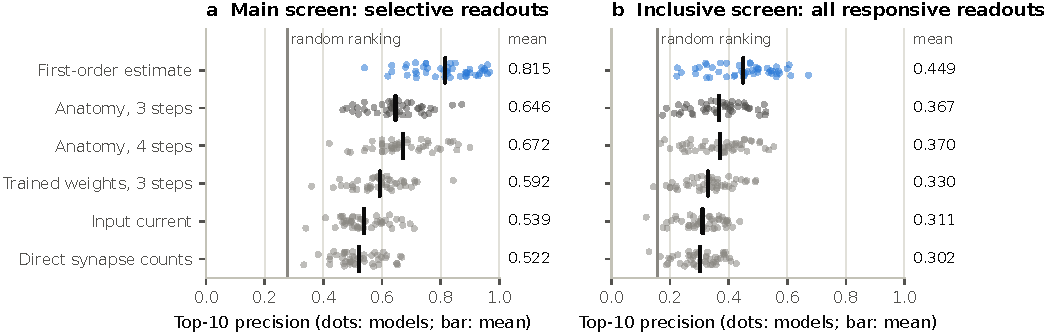
\includegraphics[width=\textwidth]{figures/s1-fig1-screening.pdf}
  \caption{Top-10 precision of each ranking at full silencing, one dot per confirmation model, with the mean as a bar and its value on the right. (a) Main screen: direction-selective readout conditions, large effect $|\Delta\DSI|\ge\LargeThreshold$. (b) Inclusive screen: all responsive readout conditions and all cell types, with abolished responses counted as large effects. The vertical line is the expected precision of a random ranking.}
  \label{fig:screen}
\end{figure}

\begin{table}[t]
  \centering
  \small
  \caption{Screening and ranking by each method, means over the \NConfModels{} confirmation models. Precision and recall refer to the ten highest-ranked cell types; Spearman $\rho$ compares each ranking with the magnitude of the exact change, over all scored cell types or over large effects only. The inclusive screen scores all responsive readout conditions and counts abolished responses as large effects. Bold: first-order estimate.}
  \label{tab:screen}
  \begin{tabular}{lcccccc}
    \toprule
    & \multicolumn{2}{c}{Top-10 precision} & Recall & \multicolumn{2}{c}{Spearman $\rho$, $s=1$} & Inclusive \\
    \cmidrule(lr){2-3}\cmidrule(lr){5-6}
    Ranking & $s=0.5$ & $s=1$ & $s=1$ & all & large & precision, $s=1$ \\
    \midrule
    \tableinput{generated/s1-table-screen.tex}
  \end{tabular}
\end{table}

Anatomical precision at full silencing rose with path length, from \PrecAnatOneFull{} for one step (the same ranking as direct synapse counts) to \PrecAnatTwoFull{}, \PrecAnatFull{} and \PrecAnatFourFull{} for two, three and four steps; graph distance reached \PrecDistFull{}. The four-step variant, the best of these, still trailed the first-order estimate by \PrecDiffAnatFourFull{} \PrecDiffAnatFourCIFull{}. Rankings that use the trained models fell below anatomy: trained-weight path weights reached \PrecTrainedFull{} and the intact input currents \PrecCurrentFull{}. Over all scored cell types, the first-order ranking agreed far more closely with the exact one than any other ranking (Spearman correlation \RhoFOFull{}, against \RhoAnatFull{} for three-step anatomy).

The inclusive screen gave \InclFOFull{} \InclFOCIFull{} for the first-order estimate and \InclAnatFull{} \InclAnatCIFull{} for three-step anatomy, against \InclRandomFull{} for a random ranking (\cref{fig:screen}b). Its precisions are lower for every method because the readout conditions with weak selectivity that it adds have few large changes: a random ranking would score \InclRandomLowDSIFull{} there and \InclRandomMainDSIFull{} in the direction-selective ones (post hoc). The paired difference was \InclDiffAnatFull{} \InclDiffAnatCIFull{}, computed post hoc with the prespecified bootstrap, and the first-order estimate was higher in \InclWinsAnatFull{} models, equal in \InclTiesAnatFull{} and lower in \InclLossesAnatFull{}.

\begin{table}[t]
  \centering
  \small
  \caption{Paired comparisons at full silencing: first-order estimate minus each ranking, means over models with 95\% bootstrap intervals, and the numbers of models in which the first-order value is higher, equal or lower (higher and lower for correlations). Correlation differences among large effects use the readout conditions in which both correlations exist (\RhoUnitsFull{} for three-step anatomy).}
  \label{tab:paired}
  \footnotesize
  \setlength{\tabcolsep}{4pt}
  \begin{tabular}{lcccc}
    \toprule
    & \multicolumn{2}{c}{Top-10 precision} & \multicolumn{2}{c}{Spearman $\rho$, large effects} \\
    \cmidrule(lr){2-3}\cmidrule(lr){4-5}
    Ranking & Difference [95\% interval] & Higher/equal/lower & Difference [95\% interval] & Higher/lower \\
    \midrule
    \tableinput{generated/s1-table-paired.tex}
  \end{tabular}
\end{table}

\subsection{The first-order estimate misjudges the size and sign of the effects}
\label{sec:effects}

\Cref{fig:s1-scatter} plots every scored case. At both strengths the estimates scatter widely around the line of equality. Pooled over cases (post hoc), the Pearson correlation between estimate and exact change was \PearsonPooledHalf{} at half strength and \PearsonPooledFull{} at full silencing; at full silencing, \LargeDecPredIncPct\% of the \LargeDecFull{} large decreases of selectivity were predicted as increases and \LargeIncPredDecPct\% of the \LargeIncFull{} large increases as decreases, and \AbsPredAboveOneFull{} estimates exceeded 1 in magnitude, a change larger than the whole range of the index allows (the largest was \MaxAbsPredFull{}).

\begin{figure}[t]
  \centering
  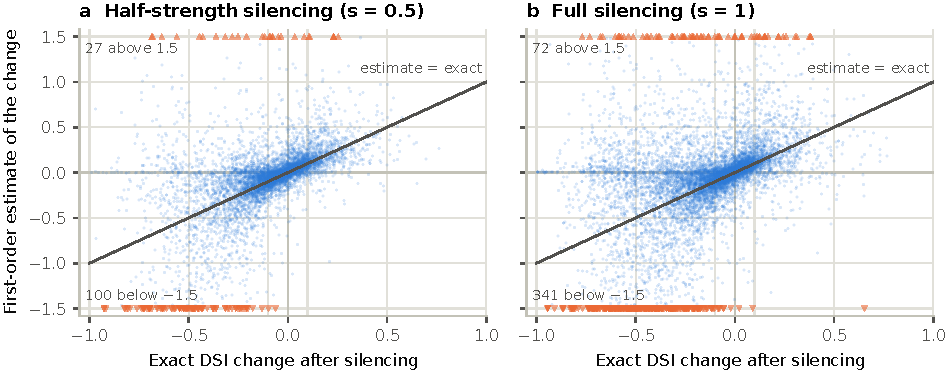
\includegraphics[width=\textwidth]{figures/s1-fig2-predicted-vs-exact.pdf}
  \caption{First-order estimate against exact change in DSI for every scored silencing case, pooled over the confirmation models: (a) \MainCasesHalf{} cases at half strength, (b) \MainCasesFull{} at full silencing. The diagonal marks equality and the grey vertical lines mark the large-effect threshold $|\Delta\DSI|=\LargeThreshold$. Estimates beyond the plotted range are drawn at its edge as triangles, with their numbers given in the panels.}
  \label{fig:s1-scatter}
\end{figure}

\Cref{tab:magnitude} gives the errors. At full silencing the mean absolute error of the first-order estimate was \MaeFOFull{} \MaeFOCIFull{}, and predicting zero change gave \MaeZeroFull{} \MaeZeroCIFull{}. The paired difference was \MaeDiffFull{} \MaeDiffCIFull{}, and the first-order error was the larger one in \MaeWorseFull{} of \NConfModels{} models (\cref{fig:errors}b; every model is listed in \cref{app:models}). The errors run in both directions: the mean signed error was \BiasFull{} \BiasCIFull{} (summarised post hoc), and it ranged from \BiasMinFull{} to \BiasMaxFull{} across models. Among the \LargeFull{} large changes (\LargeFullPct\% of scored cases) the first-order error was \MaeLargeFOFull{} against \MaeLargeZeroFull{} for zero change, and \WrongSignFull\% \WrongSignCIFull{} of the estimates had the wrong sign; the model with the fewest sign errors had \WrongSignMinFull\% and the one with the most \WrongSignMaxFull\%. Only \ZeroPredFull\% of large changes had an estimate of exactly zero, so the sign errors come from estimates pointing the wrong way rather than from missing ones.

\begin{table}[t]
  \centering
  \small
  \caption{Effect-size errors in the main analysis, means over the \NConfModels{} confirmation models with 95\% bootstrap intervals. Errors are pooled over each model's scored cases before averaging over models. The mean signed error is first-order estimate minus exact change (summarised post hoc).}
  \label{tab:magnitude}
  \begin{tabular}{lcc}
    \toprule
    & Half strength ($s=0.5$) & Full silencing ($s=1$) \\
    \midrule
    \tableinput{generated/s1-table-magnitude.tex}
  \end{tabular}
\end{table}

Clipping each estimate so that the predicted index stays in $[0,1]$ lowered the error to \MaeClipFull{}, below predicting zero change by \ClipDiffFull{} \ClipDiffCIFull{} and in \ClipBetterFull{} of \NConfModels{} models. Before clipping, \OutsideFull\% of the estimates placed the index outside its possible range. Clipping removes impossible values but leaves the wrong signs in place.

At half strength the first-order error, \MaeFOHalf{}, was close to the zero-change error, \MaeZeroHalf{} (difference \MaeDiffHalf{} \MaeDiffCIHalf{}); it was the larger error in \MaeWorseHalf{} models and the smaller in \MaeBetterHalf{}. Of the large changes, \WrongSignHalf\% had the wrong sign, and the clipped estimate reached \MaeClipHalf{}. When every responsive readout condition and every case with a defined DSI is included, the full-silencing errors were \InclMaeFOFull{} for the first-order estimate, \InclMaeZeroFull{} for zero change and \InclMaeClipFull{} for the clipped estimate (\cref{app:sensitivity}).

\begin{figure}[t]
  \centering
  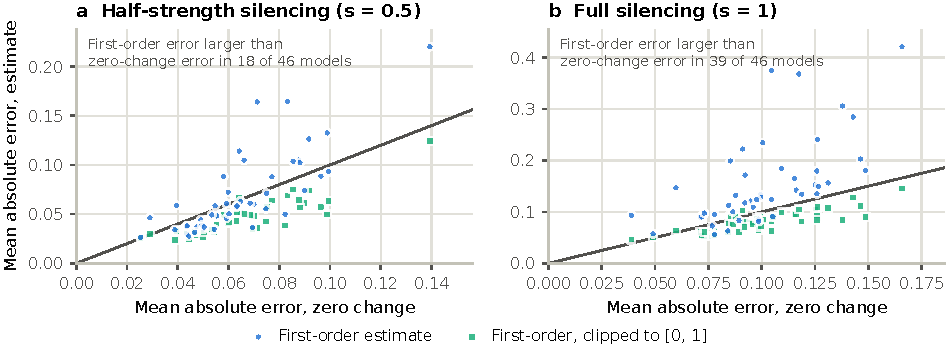
\includegraphics[width=\textwidth]{figures/s1-fig3-model-errors.pdf}
  \caption{Mean absolute error of the first-order estimate (circles) and of the clipped estimate (squares) against that of predicting zero change, one point per confirmation model: (a) half strength, (b) full silencing. Points above the diagonal are models in which the estimate is less accurate than predicting zero change.}
  \label{fig:errors}
\end{figure}

\subsection{Among large effects, the ranking is no better than anatomy}
\label{sec:ranking}

Separating large from small effects and ordering the large effects are different tasks. Among large effects only, the Spearman correlation of the first-order ranking with the exact change at full silencing was \RhoLargeFOFull{}, against \RhoLargeAnatFull{} for three-step anatomy and \RhoLargeTrainedFull{} for trained-weight path weights (\cref{tab:screen}). The paired difference from anatomy was \RhoLargeDiffAnatFull{} \RhoLargeDiffAnatCIFull{}, and the first-order estimate was higher in \RhoLargeWinsAnatFull{} of \RhoLargeModelsAnatFull{} models (\cref{tab:paired}). At half strength it ranked large effects better than anatomy (\RhoLargeFOHalf{} against \RhoLargeAnatHalf{}, difference \RhoLargeDiffAnatHalf{} \RhoLargeDiffAnatCIHalf{}; higher in \RhoLargeWinsAnatHalf{} models). Its advantage at full silencing is therefore in separating large effects from small ones.

\subsection{The error grows with silencing strength}
\label{sec:s1-strength}

The development models were also silenced at strengths 0.1, 0.25 and 0.75 (\cref{fig:s1-strength}; \cref{app:development}). The first-order error grew faster with strength than the zero-change error: it was the smaller of the two at strength 0.1 (\DevMaeFOOneTenth{} against \DevMaeZeroOneTenth{}) and 0.25 (\DevMaeFOQuarter{} against \DevMaeZeroQuarter{}) and the larger from 0.5 on, reaching \DevMaeFOFull{} against \DevMaeZeroFull{} at full silencing. It was the more accurate predictor in every development model at strength 0.1, in \DevBetterQuarter{} of \NDevModels{} at 0.25 and in none at 0.75 or 1. Screening precision rose with strength for both rankings because more changes exceed the fixed threshold, and the first-order estimate led anatomy at every strength (\DevPrecFOOneTenth{} against \DevPrecAnatOneTenth{} at 0.1, \DevPrecFOFull{} against \DevPrecAnatFull{} at 1). At full and half strength the development models agree with the confirmation results.

\begin{figure}[t]
  \centering
  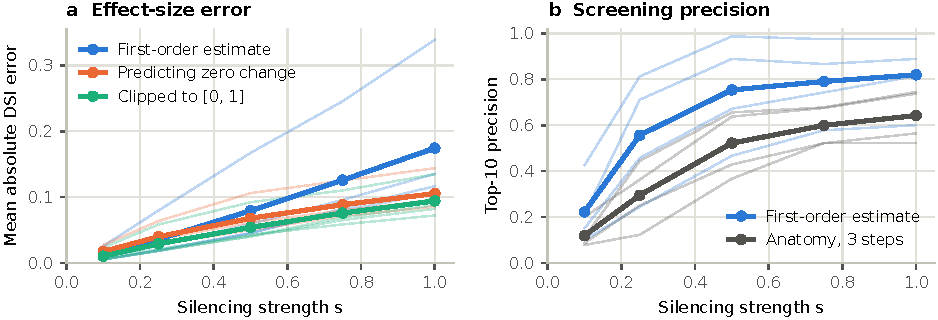
\includegraphics[width=\textwidth]{figures/s1-fig4-strength.pdf}
  \caption{Dependence on silencing strength in the four development models. (a) Mean absolute error of the first-order estimate, of predicting zero change and of the clipped estimate. (b) Top-10 precision of the first-order estimate and of three-step anatomy. Thin lines: individual models; thick lines: means. Each strength is scored on its own set of cases.}
  \label{fig:s1-strength}
\end{figure}

\subsection{Where the errors arise}
\label{sec:diagnostics}

The errors are concentrated in a minority of cases (\cref{tab:diagnostics}). For changes smaller than \LargeThreshold{} the median absolute error was \MedianErrSmallFull{}, and for large changes \MedianErrLargeFull{}. Errors were larger when the silenced type synapses directly onto the readout cell (\MaeDirectFull{}, \InputDirectCases{} cases) than when it acts only through other cells (\MaeIndirectFull{}, \InputIndirectCases{} cases). They were largest when silencing changed the set of directions that evoke no response at all, by silencing a response or by creating one (\MaeZeroPeakChangedFull{} in \ZeroPeakChangedCases{} cases, against \MaeZeroPeakSameFull{} in \ZeroPeakSameCases{} cases where that set stayed the same). The derivative is blind to such changes: a direction with a zero peak contributes zero derivative, so a response that appears is missed, and a response that disappears is extrapolated linearly past the floor of zero. In readout conditions with intact DSI below \MainDSI{}, which the main analysis leaves out, the first-order error was \MaeLowDSIFull{} against \MaeZeroLowDSIFull{} for zero change over \LowDSICasesFull{} cases. These categories overlap and describe associations; Study 2 (\cref{sec:study2}) tests where the nonlinearity lies.

\begin{table}[t]
  \centering
  \small
  \caption{Errors at full silencing by kind of case. Left: the main analysis, with the share of first-order estimates that place the index outside $[0,1]$. Right: all responsive readout conditions with a defined DSI after silencing, including amplified cases. Means over models of per-model mean absolute errors.}
  \label{tab:diagnostics}
  \footnotesize
  \setlength{\tabcolsep}{4.5pt}
  \begin{tabular}{lrcccrcc}
    \toprule
    & \multicolumn{4}{c}{Main analysis} & \multicolumn{3}{c}{All responsive} \\
    \cmidrule(lr){2-5}\cmidrule(lr){6-8}
    Cases & Number & First-order & Zero & Outside (\%) & Number & First-order & Zero \\
    \midrule
    \tableinput{generated/s1-table-diagnostics.tex}
  \end{tabular}
\end{table}

\subsection{Abolished, unchanged and amplified responses}
\label{sec:abolition}

Full silencing abolished the response of the readout in \AbolishedFull{} of the \ResponsiveCases{} cases in responsive readout conditions (\AbolishedFullPct\%), spread over \AbolitionReadoutsFull{} readout conditions; half strength abolished \AbolishedHalf{}. Silencing Mi1 caused \AbolishedByMiOne{} abolitions, L1 \AbolishedByLOne{}, Mi4 \AbolishedByMiFour{} and Tm3 \AbolishedByTmThree{} (post hoc counts). Where the response survived, its amplitude usually changed little: the median ratio of preferred-polarity peak responses after and before full silencing was \AmpRatioMedian{} (quartiles \AmpRatioQOne{} and \AmpRatioQThree{}; 5th and 95th percentiles \AmpRatioLowQ{} and \AmpRatioHighQ{}), with \AmpRatioBelowHalfPct\% of ratios below one half and \AmpRatioAboveTwoPct\% above two (post hoc). Large changes of selectivity came with larger changes of amplitude (median ratio \AmpRatioLargeMedian{}, quartiles \AmpRatioLargeQOne{} and \AmpRatioLargeQThree{}): large decreases of selectivity typically came with larger responses (median \AmpRatioLargeDecMedian{}) and large increases with smaller ones (median \AmpRatioLargeIncMedian{}; post hoc).

In \ZeroGradReadouts{} readout conditions every first-order estimate was exactly zero. Of these, \Unresponsive{} have no response at all, and in \ZeroGradResponsiveSilent{} the readout responds only to edges of the other polarity, so its DSI is 0 and its rectified peaks give zero derivative. In the remaining \ZeroGradSelective{}, all in the main analysis, a single direction of the preferred polarity evokes a response, so the DSI equals 1 whatever the size of that response; full silencing nevertheless abolished the response for \ZeroGradAbolitionsRange{} cell types in each of them (post hoc).

Amplification beyond \AmpLimit{} times the largest intact readout voltage followed \AmplifiedInterventionsFull{} full-silencing interventions (each a model, stimulus and cell type), affecting \AmplifiedCasesFull{} responsive cases, and \AmplifiedInterventionsHalf{} interventions at half strength (\AmplifiedCasesHalf{} cases); \cref{app:coverage} counts all exclusions.

\subsection{Thresholds, tuning groups and pairs}
\label{sec:robustness}

The comparison holds across the prespecified thresholds (\cref{app:sensitivity}). For the \SensCombos{} combinations of a DSI threshold of at least 0.1 with an amplification limit of \AmpLimitLow{}, \AmpLimit{}, \AmpLimitHigh{} or none, first-order precision at full silencing ranged from \SensPrecFOMin{} to \SensPrecFOMax{} and anatomical precision from \SensPrecAnatMin{} to \SensPrecAnatMax{}, and in all \SensCombosAll{} combinations, including a DSI threshold of 0, the first-order error exceeded the zero-change error. The three groups of models with upward, downward and weak T4c tuning~\citep{lappalainen2024connectome} gave the same picture (\cref{app:clusters}): first-order precision was \ClusterUpPrec{}, \ClusterDownPrec{} and \ClusterWeakPrec{}, and at full silencing the first-order error exceeded the zero-change error in each group. In the development models, silencing two input types of T4 together often changed the DSI by more or less than the sum of the single effects (median absolute interaction \PairMiOneMiFourDSI{} for Mi1 with Mi4), while pairs of T5 inputs interacted weakly (\cref{app:pairs}).

%======================================================================
\section{Study 2: why the first-order estimates fail}
\label{sec:study2}

Unless stated otherwise, results are means over the \NConfModels{} confirmation models at full strength, with 95\% bootstrap intervals over models. Study 2 recomputed the reference from its own derivatives, and it equals Study 1's saved model-level values (\RefCheckValues{} values, largest difference \RefCheckMax{}): its error ratio, the mean over models of each model's ratio of the two errors, is \RatioRefFull{} \RatioCIRefFull{}, and the mean absolute errors themselves are those of \cref{sec:effects}, \MaeFOFull{} for the reference and \MaeZeroFull{} for predicting zero change.

\subsection{Only mean replacement improves on the reference}
\label{sec:arms}

\Cref{tab:arms} and \cref{fig:ratios} give the three arms. \textbf{Mean replacement (arm~a)} lowers the error ratio to \RatioAFull{} \RatioCIAFull{}, a change of \ChangeAFull{} \ChangeCIAFull{}; it is lower than the reference in \LowerThanRefA{} of \NConfModels{} models (\cref{fig:models}). Its effects are smaller (predicting zero change has a mean absolute error of \MaeZeroAFull{} against \MaeZeroRefFull{} under silencing), and at full strength its estimate is still not distinguishable from predicting zero change (difference in mean absolute error \MaeDiffAFull{}, \MaeDiffCIAFull{}). At half strength it beats it, with an error ratio of \RatioAHalf{} \RatioCIAHalf{} (difference \MaeDiffAHalf{}, \MaeDiffCIAHalf{}). Its estimates are biased upwards (\BiasAFull{}, \BiasCIAFull{}) and give more wrong signs than the reference (\WrongAFull\%; change \WrongChangeAFull{}, \WrongChangeCIAFull{}). They still pick out the influential cell types better than anatomy (top-10 precision \TopTenAFull{} against \AnatAFull{}).

\begin{table}[t]
\centering
\caption{The reference and the three arms of Study 2. Error ratio: mean absolute error divided by that of predicting zero change on the same cases (below 1 is better than predicting zero change). Change: paired difference in error ratio from the reference. Against zero change: decision on the interval for the difference in mean absolute error. Wrong signs: fraction of large effects estimated with the opposite sign. Top-10: precision of the ten largest estimates, with anatomy (three synaptic steps) on the same cases in brackets. Means over \NConfModels{} models with 95\% bootstrap intervals.}
\label{tab:arms}
\footnotesize
\setlength{\tabcolsep}{3pt}
\begin{tabular}{@{}llllllll@{}}
\toprule
Estimate & $s$ & Error ratio & Change & \makecell[l]{Against\\ zero change} & \makecell[l]{Signed\\ error} & \makecell[l]{Wrong\\ signs} & \makecell[l]{Top-10\\ (anatomy)} \\
\midrule
\tableinput{generated/s2-table-arms.tex}
\bottomrule
\end{tabular}
\end{table}

\begin{figure}[t]
\centering
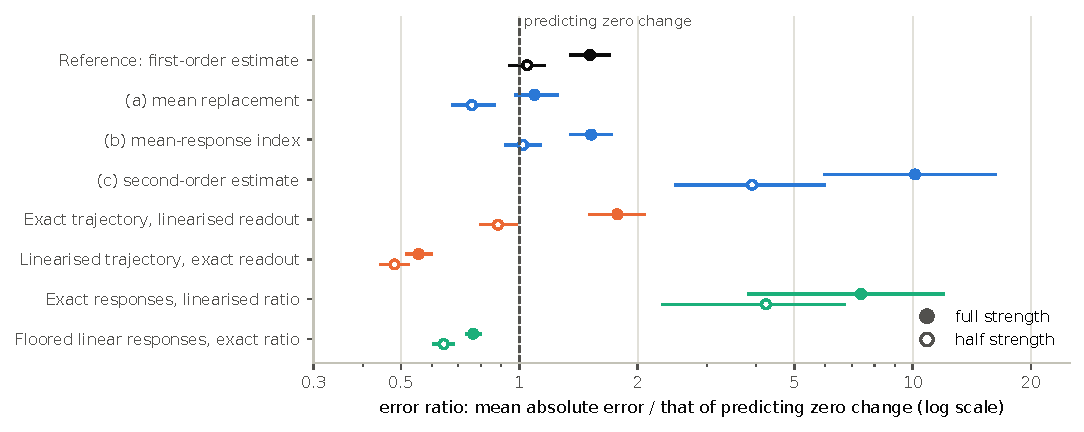
\includegraphics[width=\linewidth]{figures/s2-fig1-error-ratios.pdf}
\caption{Error ratio of every estimator of Study 2 in the \NConfModels{} confirmation models, at full strength (filled) and half strength (open), with 95\% bootstrap intervals over models. Black: the reference, Study 1's first-order estimate. Blue: the three arms, each changing one thing. Orange: the exact readout applied to the linearised trajectory, and the linearised readout applied to the exact trajectory. Green: the two stages of the readout, one exact and one linearised, on the linearised trajectory.}
\label{fig:ratios}
\end{figure}

\textbf{The mean-response index (arm~b)} changes nothing detectable: error ratio \RatioBFull{} \RatioCIBFull{}, change \ChangeBFull{} \ChangeCIBFull{}, and its estimate is worse than predicting zero change (\MaeDiffBFull{}, \MaeDiffCIBFull{}). It gives fewer wrong signs (\WrongBFull\%; change \WrongChangeBFull{}, \WrongChangeCIBFull{}) and screens as well as the peak index (\TopTenBFull{} against \AnatBFull{}).

\textbf{The second-order estimate (arm~c)} is far worse than the first-order one: error ratio \RatioCFull{} \RatioCICFull{}, with a large upward bias (\BiasCFull{}, \BiasCICFull{}) and \WrongCFull\% wrong signs. It changes the ranking little (top-10 precision \TopFirstCFull{} from first order, \TopFirstCICFull{}). By the prespecified rule, mean replacement dominates, because it is the only arm that improves on the reference.

\begin{figure}[t]
\centering
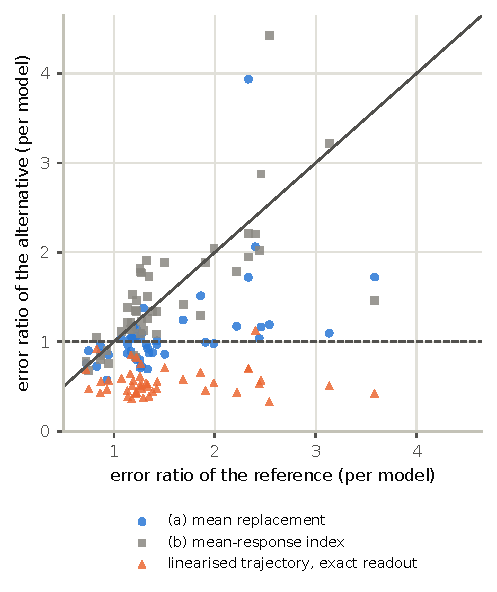
\includegraphics[width=0.56\linewidth]{figures/s2-fig3-per-model.pdf}
\caption{Per-model error ratios at full strength: arm~(a), arm~(b) and the exact readout on the linearised trajectory, against the reference. Solid line: equal error ratios; dashed line: predicting zero change.}
\label{fig:models}
\end{figure}

\subsection{The nonlinearity is in the readout}
\label{sec:mechanism}

\begin{table}[t]
\centering
\caption{Where the nonlinearity lies (silencing, peak index, full strength). Share of error removed: $1-\mathrm{MAE}/\mathrm{MAE}_{\text{first order}}$ per model. Against zero change: mean absolute error minus that of predicting zero change. Means over \NConfModels{} models with 95\% bootstrap intervals.}
\label{tab:mechanism}
\footnotesize
\setlength{\tabcolsep}{3pt}
\begin{tabularx}{\linewidth}{@{}Ylllr@{}}
\toprule
Estimator & Error ratio & Share of error removed & Against zero change & Wrong signs \\
\midrule
\tableinput{generated/s2-table-mechanism.tex}
\bottomrule
\end{tabularx}
\end{table}

\enlargethispage{\baselineskip}\Cref{tab:mechanism} gives the estimators of \cref{sec:counterfactual}. Applying the linearised readout to the exactly simulated trajectories does not help: its error ratio is \RatioCfNetFull{} \RatioCICfNetFull{}, and it removes \RecNetZPFull\% of the first-order error, that is, it adds error. Applying the exact readout to the linearised trajectory removes \RecReadZPFull\%: its error ratio is \RatioCfReadFull{} \RatioCICfReadFull{}, below 1 in \BelowOneCfRead{} of \NConfModels{} models, it beats predicting zero change (difference \MaeDiffCfReadFull{}, \MaeDiffCICfReadFull{}), and only \WrongCfReadFull\% of large effects get the wrong sign. The readout's nonlinearity, not the network's, accounts for Study 1's error (difference in error removed \ReadMinusNetZPFull{}, \ReadMinusNetCIZPFull{}). \Cref{fig:s2-scatter} shows the difference case by case. The same holds for the mean-response index (\RecReadZMFull\% against \RecNetZMFull\%) and under mean replacement (\RecReadMPFull\% against \RecNetMPFull\%; \cref{app:tables}).

The network's trajectories are themselves not linear: the linear approximation misses \TraceLinZero\% of the change in the readout traces (median per model), and adding the second derivative reduces this only to \TraceQuadZero\% (median ratio of the two errors \TraceRatioZero{}). These errors matter much less than the readout's because the index turns each trace into one response and then divides.

\begin{figure}[t]
\centering
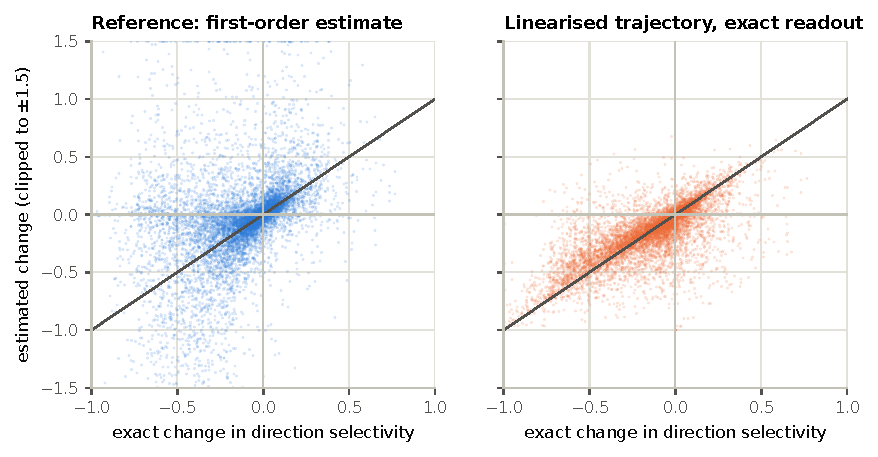
\includegraphics[width=\linewidth]{figures/s2-fig2-predicted-vs-exact.pdf}
\caption{Estimated against exact change in direction selectivity for all \PostCases{} scored silencing cases of the confirmation models at full strength (post hoc case file). Left: the reference, the estimates of \cref{fig:s1-scatter}b. Right: the exact readout applied to the linearised trajectory. Estimates are clipped to $\pm1.5$ for display; the line marks equality.}
\label{fig:s2-scatter}
\end{figure}

\subsection{Within the readout, the ratio}
\label{sec:split}

The split of Amendment~1 separates the two stages of the readout on the linearised trajectory (\cref{tab:mechanism}, green in \cref{fig:ratios}). Applying the exact ratio to the floored linear responses removes \RecRatioZPFull\% of the first-order error: its error ratio is \RatioSplitRatioFull{} \RatioCISplitRatioFull{}, below 1 in \BelowOneSplitRatio{} of \NConfModels{} models, and it beats predicting zero change (\MaeDiffSplitRatioFull{}, \MaeDiffCISplitRatioFull{}). Making only the responses exact and linearising the ratio makes the estimate far worse (error ratio \RatioSplitRespFull{} \RatioCISplitRespFull{}): a linearised ratio applied to large changes of the responses overshoots, as the second-order term does. The ratio stage dominates (difference in error removed \RatioMinusRespZPFull{}, \RatioMinusRespCIZPFull{}). With the mean-response index, whose response stage is the rectification alone, the pattern is the same (\RecRatioZMFull\% removed by the exact ratio against \RecRespZMFull\% by exact responses). The two stages interact strongly: making both exact removes more than the two single changes added together (\InteractionZPFull{}, \InteractionCIZPFull{}), so neither stage alone accounts for the whole effect.

\subsection{Why the second-order estimate overshoots}
\label{sec:second}

This subsection is post hoc. Splitting the second-order term of \cref{eq:second} into the network's part, $\tfrac12 s^2\,\nabla F\cdot K$, and the readout's curvature, $\tfrac12 s^2\,J^{\top}(\nabla^2F)J$, the readout's part makes up \PostShareReadout\% of the term's absolute size (mean over models). The term is concentrated in the cases where the linearised trajectory changes the index's denominator by more than its own size: these are \PostLargeDenFrac\% of cases but carry \PostLargeDenShare\% of the term. The Taylor series of a ratio in the strength converges only while the denominator's change stays below the denominator itself, so in these cases the second-order term diverges. Their mean absolute error is \PostLargeSecond{} for the second-order estimate, \PostLargeFirst{} for the first-order estimate and \PostLargeZero{} for predicting zero change. In the remaining cases the first-order estimate is about as good as predicting zero change (\PostRestFirst{} against \PostRestZero{}), and the second-order estimate is worse (\PostRestSecond{}); it beats the first-order estimate in \PostRestSecondBelowFirst{} of \NConfModels{} models. The curvature available to a second-order correction therefore does not repair the estimate anywhere in these models, and Study 1's failure lies mostly in the cases where silencing changes the response by a large fraction.

\subsection{Strength}
\label{sec:s2-strength}

In the development models (\cref{tab:s2-development}), the reference's error ratio rises from \DevRefPointOne{} at strength 0.1 to \DevRefFull{} at full silencing and passes 1 between strengths 0.25 and 0.5, as Study 1's errors do (\cref{fig:s1-strength}). Under mean replacement it stays below 1 up to strength 0.75 (\DevAThreeQ{}). The exact readout on the linearised trajectory stays below 1 at every strength (\DevCfReadPointOne{} to \DevCfReadFull{}), and the second-order estimate is worse than the first-order one at every strength. In the confirmation models at half strength, the reference's error ratio is \RatioRefHalf{} \RatioCIRefHalf{} and the exact readout on the linearised trajectory reaches \RatioCfReadHalf{} \RatioCICfReadHalf{}.

\subsection{Baseline mismatch}
\label{sec:mismatch}

Using the silencing derivative to estimate the effects of mean replacement gives an error ratio of \RatioMisMeanFull{} \RatioCIMisMeanFull{}, \MisMeanMinusMatchedFull{} \MisMeanMinusMatchedCIFull{} above the matched estimate, and it loses its advantage in screening: its top-10 precision, \TopTenMisMeanFull{}, equals that of anatomy (\AnatMisMeanFull{}; difference \MisMeanTopAnatFull{}, \MisMeanTopAnatCIFull{}). In the other direction, the derivative of mean replacement estimates the effects of silencing with an error ratio of \RatioMisZeroFull{} \RatioCIMisZeroFull{}, lower than the silencing derivative's own (difference \MisZeroMinusRefFull{}, \MisZeroMinusRefCIFull{}).

\subsection{The predictions}
\label{sec:predictions}

Of the \PredPrimaryTotal{} predictions hashed before the development phase, \PredPrimaryHeld{} hold (\cref{app:predictions}). The failures are the size of arm~(c)'s failure (error ratio and wrong-sign rate far above the predicted ranges, and its bias beyond the predicted bound), arm~(a)'s wrong-sign rate (higher than predicted), and the expectation that the mismatched silencing derivative would keep its screening advantage. Of the \PredAddendumTotal{} predictions informed by the development results, \PredAddendumHeld{} hold; the exception is that arm~(b) was predicted to be worse than the reference and is not detectably different.

%======================================================================
\section{Computational cost}
\label{sec:cost}

Per model and for both stimuli, exact silencing of the \SimulatedTypes{} cell types with a path to the readouts took \TimeExactFull{}~s at one strength and \TimeExactBoth{}~s at both strengths, and Study 1's first-order estimates for the eight readouts took \TimeGradient{}~s: \TimeForward{}~s for the forward pass and \TimeBackwardEach{}~s for each readout's backward pass. Exact silencing at one strength was thus slightly faster (model-mean time ratio \TimeRatioFull{}), and at two strengths it took \TimeRatioBoth{} times as long. The two costs scale with different quantities. Exact silencing costs one simulation per intervention, about \TimePerType{}~s per cell type and strength here. The first-order estimate costs one backward pass per readout, about as much as \BackwardOverType{} silencing simulations, and serves every strength at once. It saves computation only when the interventions of interest outnumber the readouts by more than this factor; with \SimulatedTypes{} cell types and eight readouts, the FlyVis models are close to the break-even point. These timings cover the simulation and differentiation on one 6 GB NVIDIA GPU (single precision, \BatchSize{} silencing simulations per batch) and exclude model loading, adaptation to the grey screen and file input and output.

Study 2's forward recursions for the first and second derivatives of all \NSimTypes{} cell types took \TimeTangentsZero{}~s per model on the GPU, \TimeRatioTangents{} times as long as exact silencing of all of them at one strength. Exact mean replacement took \TimeRatioExactMean{} times as long as exact silencing. Study 2 also prespecified a practical rule: screen with Study 1's derivatives, simulate the \FlagBudgetPrimary{} cell types with the largest estimates for each stimulus, and predict zero change for the rest. It removes \FlagRecTenZero\% of the error of predicting zero change in \FlagSecTenZero{}~s per model. That is \FlagPerSecTenZero{} of the error per second, against \ExhaustivePerSec{} per second for simulating every cell type, so the rule never pays in these models at any of the budgets tried (\cref{app:tables}).

%======================================================================
\section{Related work}
\label{sec:related}

\paragraph{First- and second-order removal estimates.}
\citet{mozer1989skeletonization} estimated the relevance of a unit from the derivative of the network's error with respect to a gain on the unit's output, the construction we evaluate here with silencing strength as the gain. Optimal brain damage and optimal brain surgeon used the diagonal or the full Hessian of the loss instead~\citep{lecun1990optimal,hassibi1993second}, and \citet{molchanov2017pruning,molchanov2019importance} ranked convolutional filters and neurons for pruning with first- and second-order Taylor expansions of the loss. In pruning the estimate has to rank components; our question is whether it also gives the size and sign of each effect, and if not, why not.

\paragraph{Attribution patching.}
In language models, attribution patching approximates activation patching to first order~\citep{nanda2023attribution}. Edge attribution patching recovered circuits better than earlier automated methods~\citep{syed2024attribution}. \citet{kramar2024atp} identified two kinds of failure that cause false negatives, saturated attention and cancellation, and addressed the first by computing the change of the attention softmax exactly instead of linearising it when queries and keys are patched. That repair is of the same kind as the estimator that works best in Study 2, which keeps the inputs to a normalising step linear and applies the normalisation exactly. \citet{hanna2024faith} found that circuits chosen with integrated gradients~\citep{sundararajan2017axiomatic} are more faithful than those chosen with plain attribution patching. Attribution patching can lose the size of the effects almost entirely: for the outputs of the MLP layers of GPT-2 Large in the indirect-object identification task, \citet{jafari2025relp} found a Pearson correlation of 0.006 between attribution and activation patching, and proposed replacing the local gradients with coefficients from layer-wise relevance propagation. \citet{zhang2026attribution} traced the dominant error of attribution patching to nonlinearities downstream of the patched component and proposed a second-order correction computed with Hessian-vector products, and a workflow that screens with first-order estimates and spends further computation only on the components flagged as unreliable. In the FlyVis models that correction makes the estimates worse, because the curvature it adds comes mostly from a ratio whose Taylor series diverges for large perturbations, and because it cannot see the network's threshold crossings. Our setting differs from these studies in three ways: the network is recurrent and the output is a peak-based tuning index, the intervention silences a whole cell type, and the exact effect of every intervention is known, so effect-size errors can be measured directly.

\paragraph{Baselines and attribution in the FlyVis models.}
The value that replaces a component's output (zero, a mean, or a resampled value) changes what patching experiments find~\citep{heimersheim2024patching,miller2024metrics}, and \citet{heimersheim2024patching} discuss how the choice of metric, for example a logit difference against a probability, affects the conclusions. In work concurrent with ours, \citet{dhawan2026flyhack} scored integrated gradients and edge attribution patching against exhaustive interventions on each type-to-type connection in ten of the FlyVis models, with decoded optic flow as the output. Both methods ranked the important connections highly whatever value replaced a removed connection, but they ranked the sizes of the effects well only when built for the same intervention as the reference: against the effects of mean replacement, edge attribution patching reached a Spearman correlation of 0.872 when built for mean replacement and 0.126 when built for zero replacement. That study scores ranks and classification. In Study 1 the estimate and the reference share one intervention, so the effect-size errors come from nonlinearity rather than from a mismatch of baselines, and we measure absolute and signed errors against predicting zero change, how they change with silencing strength, and the cost of each method. In Study 2, changing the shared baseline to each cell's mean output reduces the error but does not remove it, and a mismatched derivative loses both the effect sizes and the screening advantage.

\paragraph{Connectome-constrained models of the fly visual system.}
\citet{lappalainen2024connectome} trained the FlyVis ensemble and described groups of models with different T4c tuning. During peer review they simulated silencing of Mi1, Tm3, Mi4 and Mi9 by clamping each type's outputs to zero, averaged the T4c responses over the models with correct T4c tuning, and reported qualitative agreement with the experiments of \citet{strother2017emergence} for most effects~\citep{lappalainen2024review}. \citet{ryan2026silencing} silenced cell types in the same \NModels{} models and compared the effects with published results of genetic silencing, under a protocol fixed before any outcome was coded: the ensemble's predictions agreed with the experiments better than chance but no better than a baseline built from synapse counts alone, which, like our anatomical path weights, follows paths of up to three synaptic steps back from the readout. Later studies in the same series simulated every single cell type and every pair, and samples of up to five types together, in every model~\citep{ryan2026tests,ryan2026budget}; there, a linear model of the signed connectome ranked the magnitudes of the interactions between silenced types but predicted their signs at or below chance~\citep{ryan2026budget}, a split between locating effects and estimating them like the one we find for first-order estimates. \citet{dhiman2026scale} silenced T4 and T5 in a FlyVis model and found that a refitted linear decoder still recovered the direction of motion. \citet{karaneen2026reproducibility} retrained ensembles of such models and found that selecting models by task error does not reliably identify the solutions that match measured tuning. \citet{pospisil2024effectome} proposed estimating a linear causal model of the fly brain from optogenetic perturbations, with the connectome as a prior; our anatomical path weights use the connectome alone in a related way. \citet{xie2025visual} predicted the visual responses of neurons across the fly brain by aggregating paths through powers of the connectome's adjacency matrix, a construction close to our path weights.

\paragraph{Biological silencing.}
Genetic silencing experiments characterised the inputs of the ON motion detector T4, Mi1, Tm3, Mi4 and Mi9~\citep{ammer2015functional,strother2017emergence}, and of the OFF motion detector T5, Tm1, Tm2, Tm4 and Tm9~\citep{serbe2016comprehensive}; \citet{borst2020fly} review the circuit. Inhibition relayed by CT1 shapes the tuning of T5~\citep{braun2023disynaptic}, and the feedback neurons C2 and C3 take part in motion processing~\citep{henning2026inhibitory}. These experiments measure other quantities in other cells, by calcium imaging or electrophysiology, after silencing that lasts much longer than ours, so we use them as context only (\cref{app:biology}). Elsewhere in the fly brain, silencing in a connectome model has been tested against experiments: in a leaky integrate-and-fire model of the whole central brain, \citet{shiu2024drosophila} silenced neurons one at a time and tested several of the predicted effects on feeding by optogenetic silencing in flies.

%======================================================================
\section{Discussion}
\label{sec:discussion}

\paragraph{Screening and estimation are different tasks.}
\enlargethispage{\baselineskip}In the same cases, the first-order estimate was the best screen we tested and a worse predictor of effect size than zero change. A screen needs only the cell types with large effects to have the largest derivatives. An estimate of the effect needs the response to stay nearly linear all the way from the intact to the silenced network, and fully silencing a cell type with a large effect often takes it well beyond that range. At half strength the screen's lead over anatomy grew while the effect-size error only matched that of zero change, and in the development models the estimate beat zero change only up to strength \DevBetterMaxStrength{}.

\paragraph{The nonlinearity is in the readout.}
Study 1 found the errors concentrated where silencing changed which directions evoke a response, and where the silenced type connects directly to the readout (\cref{tab:diagnostics}). The index is built from rectified peak responses: a direction that evokes no response contributes zero derivative, so the estimate misses responses that silencing creates and extrapolates those it removes linearly past zero. Study 2 located the cause. Keeping the network's response linear costs little: the exact index applied to the linearised trajectories beats predicting zero change, with an error ratio below 1 in \BelowOneCfRead{} of \NConfModels{} models. Linearising the index is what fails, and within the index the ratio of a vector length to a sum of responses matters most. The three single changes behave accordingly. Building the index from mean responses leaves the ratio in place and changes nothing detectable. Mean replacement shrinks the perturbation and with it the change of the ratio's denominator, which lowers the error without removing it. A second-order correction adds the ratio's curvature exactly where the ratio's Taylor series diverges, and makes the estimates far worse. \Citet{zhang2026attribution} reached a related conclusion for attribution patching in language models: most of the error comes from nonlinearities between the intervention and the output.

\paragraph{Using first-order estimates.}
For choosing which cell types to silence in a model like FlyVis, the first-order ranking is a better guide than connectivity. The sizes and signs of the chosen types' effects should then be simulated, as in the screen-then-recompute workflow of \citet{zhang2026attribution}. This advice is for silencing, which drives a type's output towards zero; for mean replacement, \citet{dhawan2026flyhack} found that estimates built for that intervention rank the sizes of its effects well, and in Study 2 the matched mean-replacement estimate beat predicting zero change at half strength. Where an estimate has to serve, clipping it to the range of the index is a minimal correction: it brought the error below that of zero change in \ClipBetterFull{} of \NConfModels{} models and left the wrong signs in place. A better correction follows from Study 2. The first-order estimate of a ratio is accurate only while the perturbation changes the denominator by a small fraction of itself, and silencing a cell type can change a motion detector's summed response by more than its own size (on the linearised trajectory, in \PostLargeDenFrac\% of cases here). For such outputs the ratio should be applied exactly to linearised inputs, or the numerator and denominator reported separately. This needs the derivatives of the \NTrajectories{} responses of each readout rather than of the index alone, and so more backward passes. Second-order corrections should be avoided for ratio outputs under large perturbations, because they inherit the divergence of the ratio's series.

The cost argument for the estimate is weak at this scale. It costs one backward pass per output, against one simulation per intervention for exact silencing, so it pays off when the interventions far outnumber the outputs, as for the many components and single output of attribution patching in language models. With \SimulatedTypes{} silencing targets and eight outputs, FlyVis is close to the break-even point, exact silencing gives the right answer, and screening a few cell types before simulating them never paid (\cref{sec:cost}).

\paragraph{The same structure in language models.}
Many outputs of language models used in patching experiments are ratios: probabilities are normalised by a softmax, and attention weights by another. The repair of attribution patching for saturated attention in \citet{kramar2024atp}, which recomputes the softmax exactly, follows the same principle as the estimator that works best here. Whether the error of attribution patching in language models comes mostly from such normalisations, or from the network between them, can be tested with the same two estimators used here, which need only one exact and one linearised forward pass per component.

\needspace{5\baselineskip}
\paragraph{Limitations.}
\begin{itemize}
  \item All \NModels{} models share one connectome, one training task and one model structure, so the intervals describe variation within this released ensemble rather than across architectures or animals.
  \item We tested moving edges at two speeds and the central T4 and T5 cells, with one family of direction-selectivity indices; other stimuli, such as natural scenes, and other outputs could give the estimate a different accuracy.
  \item Study 1's main screen is scored on cases selected after silencing, because abolished and amplified responses are excluded; the inclusive screen, which keeps every responsive readout condition and cell type, gives lower precisions with the same order of methods (\cref{sec:screening}).
  \item The index depends on peaks of rectified responses; at tied peaks the derivative depends on a tie convention, and near ties occurred in \NearTieReadouts{} of \ReadoutConditions{} readout conditions.
  \item Study 2 was designed after Study 1's results were known. Its arms~(b) and~(c), the analysis of where the nonlinearity lies and the flag rule were computed from Study 1's saved simulations of the confirmation models, which Study 1 had already analysed; they were prespecified but are not blind confirmations. The split of the readout into its two stages and a second set of predictions were added after Study 2's development results were read, before its freeze. The explanation of the second-order failure in \cref{sec:second} is post hoc.
  \item The second-order term is the one automatic differentiation gives, which treats every rectifier as linear; a finite-difference term would include threshold crossings at a chosen step size. Integrated gradients along each cell type's own silencing path~\citep{sundararajan2017axiomatic} converge to the exact change, but each cell type then needs several simulations and backward passes, more than the single simulation they would replace. Mean replacement used each cell's average over the stimulus set; other averages are possible.
  \item Silencing in the model scales a type's synaptic output for the duration of one stimulus (at most \WindowSlow{}~s); genetic silencing in flies acts for longer and through other mechanisms, so the biological comparisons in \cref{app:biology} are qualitative.
\end{itemize}

%======================================================================
\section{Conclusion}
\label{sec:conclusion}

In the \NModels{} FlyVis models, first-order estimates of cell-type silencing are a good screen: they pick out the cell types whose silencing changes the direction selectivity of T4 and T5 more reliably than any ranking from connectivity, trained weights or input currents that we tested. They are a poor estimate of the effect itself. At full silencing their errors exceed those of predicting zero change, a fifth of large effects get the wrong sign, and among large effects their ranking is no better than that of anatomy. The cause is the readout, not the network: applying the index exactly to the linearised trajectories beats predicting zero change, and within the index the ratio matters most. A second-order correction makes the estimates worse, and mean replacement, a smaller perturbation, lowers the error without removing it. At this scale exact silencing costs about as much as the estimate, and when the size or sign of the effect of driving a cell type's output towards zero matters, it should be simulated.

\paragraph{Code and data availability.}
\enlargethispage{\baselineskip}The code, frozen protocols and records of both studies, the saved outputs from which every number, table and figure in this paper is computed, and the paper's source are available at \url{https://github.com/Jeevash23/interp-flyvis-first-order}. The simulated voltage traces are not included because of their size; the released code computes them again from the public FlyVis models. All of Study 1's saved responses were rechecked from their traces, one silencing case per model was replayed with the original FlyVis implementation, and Study 2 checked every confirmation model against Study 1's saved records before using its outcomes (\cref{app:verification}).


% The same statement, in the same place, in every paper of the set.
\paragraph{Use of AI assistants.}
Language-model assistants were used throughout this work, under the author's direction, to help design the studies, to write and run the code for the experiments and analyses, to draft and revise the text and to check the references against their online records. All reported results come from the saved study outputs, and the numbers in the text were generated from those outputs or checked against them.

\FloatBarrier
\bibliographystyle{plainnat}
\bibliography{references}

\appendix
% The appendix has little text between its tables: let the tables float past section headings and share pages.
\let\FloatBarrier\relax
\crefalias{section}{appendix}
\renewcommand{\floatpagefraction}{0.6}
\renewcommand{\bottomfraction}{0.9}
%======================================================================
\section{Scored cases and exclusions}
\label{app:coverage}

\Cref{tab:coverage} accounts for every confirmation readout condition and silencing case. Readout conditions are the same at both strengths; abolition and amplification depend on the strength. The \ZeroGradReadouts{} readout conditions whose first-order estimates are all exactly zero are discussed in \cref{sec:abolition}.

\begin{table}[btp]
  \centering
  \small
  \caption{Readout conditions and silencing cases in the \NConfModels{} confirmation models. A case is one cell type silenced at one strength and evaluated at one readout condition (\NetTypes{} cases per readout condition). The main analysis scores cases in direction-selective readout conditions (intact DSI at least \MainDSI{}) whose DSI after silencing is defined and whose readout voltages stay below \AmpLimit{} times the largest intact readout voltage.}
  \label{tab:coverage}
  \begin{tabular}{lcc}
    \toprule
    & Half strength & Full silencing \\
    \midrule
    \tableinput{generated/s1-table-coverage.tex}
  \end{tabular}
\end{table}

%======================================================================
\section{Sensitivity to the thresholds}
\label{app:sensitivity}

\Cref{tab:sensitivity} repeats Study 1's main comparisons at full silencing for every combination of the prespecified DSI thresholds and amplification limits. Precision rises with the DSI threshold for both rankings, because direction-selective readouts have more large changes. In every row the first-order estimate leads anatomy, and the errors are ordered the same way: clipped estimate, then zero change, then first-order estimate. With a DSI threshold of 0 and no amplification limit, the columns with abolitions reproduce the inclusive screen.

\begin{table}[btp]
  \centering
  \footnotesize
  \setlength{\tabcolsep}{3.6pt}
  \caption{Full-silencing results for each combination of minimum intact DSI and amplification limit (\emph{none}: no limit), means over the \NConfModels{} confirmation models. Precision counts large changes among the ten highest-ranked cell types; the columns marked \emph{with abolitions} also score abolished responses and count them as large effects. Bold: the prespecified main analysis.}
  \label{tab:sensitivity}
  \begin{tabular}{ccrrcccccccc}
    \toprule
    & & & & \multicolumn{2}{c}{Top-10 precision} & \multicolumn{2}{c}{With abolitions} & \multicolumn{3}{c}{Mean absolute error} \\
    \cmidrule(lr){5-6}\cmidrule(lr){7-8}\cmidrule(lr){9-11}
    Min.\ DSI & Amp.\ limit & Readouts & Cases & First-order & Anatomy & First-order & Anatomy & First-order & Zero & Clipped \\
    \midrule
    \tableinput{generated/s1-table-sensitivity.tex}
  \end{tabular}
\end{table}

%======================================================================
\section{Tuning groups}
\label{app:clusters}

\citet{lappalainen2024connectome} grouped the released models by the tuning of T4c: in the confirmation set, \ClusterUpModels{} prefer upward motion, \ClusterDownModels{} downward motion and \ClusterWeakModels{} are weakly tuned (\cref{tab:clusters}). The first-order estimate screened well in all three groups. At full silencing its error exceeded that of zero change in every group; at half strength it was slightly smaller in the upward-tuned group (\ClusterUpMaeFOHalf{} against \ClusterUpMaeZeroHalf{}) and larger in the other two. Errors were largest in the downward and weakly tuned groups, whose T4c tuning differs from that measured in flies; the group describes T4c only, and a model's other seven readouts can be tuned well or poorly.

\begin{table}[btp]
  \centering
  \small
  \caption{Study 1's main results by T4c tuning group, means over the confirmation models in each group.}
  \label{tab:clusters}
  \begin{tabular}{clcccccc}
    \toprule
    & & & Top-10 & \multicolumn{3}{c}{Mean absolute error} \\
    \cmidrule(lr){5-7}
    $s$ & T4c tuning & Models & precision & First-order & Zero & Clipped \\
    \midrule
    \tableinput{generated/s1-table-clusters.tex}
  \end{tabular}
\end{table}

%======================================================================
\section{Development models across strengths}
\label{app:development}

The four development models were silenced at five strengths on the same stimuli as the confirmation models. Each strength is scored on its own cases, because the set of large changes, abolitions and amplified responses changes with strength. With four models, the tables give means, and Study 1's table also ranges, rather than intervals. \Cref{tab:s1-development} gives Study 1's measures and \cref{tab:s2-development} the error ratios of Study 2's estimators.

\begin{table}[btp]
  \centering
  \small
  \setlength{\tabcolsep}{4.5pt}
  \caption{Study 1 in the development models (\DevModelList{}) at five silencing strengths: top-10 precision of the first-order estimate and of three-step anatomy, the Spearman correlation of the first-order ranking among large effects, mean absolute errors, the difference between first-order and zero-change errors (mean and range over the four models) and the percentage of large changes predicted with the wrong sign.}
  \label{tab:s1-development}
  \begin{tabular}{cccccccccc}
    \toprule
    & \multicolumn{2}{c}{Top-10 precision} & & \multicolumn{3}{c}{Mean absolute error} & First-order & Wrong \\
    \cmidrule(lr){2-3}\cmidrule(lr){5-7}
    $s$ & First-order & Anatomy & $\rho$, large & First-order & Zero & Clipped & minus zero [range] & sign (\%) \\
    \midrule
    \tableinput{generated/s1-table-development.tex}
  \end{tabular}
\end{table}

\begin{table}[btp]
\centering
\caption{Error ratios of Study 2's estimators across five strengths in the four development models (means over models).}
\label{tab:s2-development}
\small
\begin{tabular}{@{}llllll@{}}
\toprule
& \multicolumn{5}{c}{Silencing strength $s$} \\
\cmidrule(l){2-6}
Estimator & 0.1 & 0.25 & 0.5 & 0.75 & 1 \\
\midrule
\tableinput{generated/s2-table-development.tex}
\bottomrule
\end{tabular}
\end{table}

%======================================================================
\section{Pairs of silenced cell types}
\label{app:pairs}

The earlier four-model study silenced eight pairs of input types to T4 and T5 together, on its own stimuli. For each pair we compare the joint effect with the sum of the two single effects: the interaction is the joint change minus both single changes, computed on the DSI and, separately, on the mean voltage of each preferred-polarity response. \Cref{tab:pairs} summarises the interactions at full silencing in the direction-selective readout conditions, as medians with quartiles over readout conditions (post hoc quartiles). The pairs of T4 inputs interact strongly on the DSI, most of all Mi1 with Mi4 (median absolute interaction \PairMiOneMiFourDSI{}), while the pairs of T5 inputs interact weakly (medians at most \PairTmMaxDSI{}). When both single effects had the same sign, the joint effect was usually smaller than their sum: in most such readout conditions for every pair of T4 inputs, and for \PairTmSubadditiveMajority{} of the \PairTmCount{} pairs of T5 inputs. A bounded index can produce such subadditivity by itself, so these interactions describe the models' output rather than identify interacting circuit elements.

\begin{table}[btp]
  \centering
  \footnotesize
  \setlength{\tabcolsep}{4pt}
  \caption{Interactions between pairs of silenced cell types at full silencing in the development models, median [quartiles] over direction-selective readout conditions. Voltage interactions are root-mean-square values over the preferred-polarity stimuli in model units; the relative value divides by the sum of the two single effects' root-mean-square values. Last column: readout conditions with a subadditive DSI change among those whose two single effects have the same sign.}
  \label{tab:pairs}
  \begin{tabular}{lccccc}
    \toprule
    Pair & Readouts (models) & $|$DSI interaction$|$ & Voltage interaction & Relative voltage & Subadditive \\
    \midrule
    \tableinput{generated/s1-table-pairs.tex}
  \end{tabular}
\end{table}

%======================================================================
\section{Biological context}
\label{app:biology}

\Cref{tab:biology} lists, for the four development models and the fast stimulus, the effect of fully silencing cell types that have been silenced in flies. The amplitude ratio compares the summed preferred-polarity peak responses after and before silencing. Silencing Mi1 abolished the responses of T4 in most readout conditions (DSI defined after silencing in \BioMiOneTFourDefined{} of \BioMiOneTFourConditions{}), and silencing Tm3 reduced them (median ratio \BioTmThreeTFourRatio{}). These two results agree in direction with the silencing simulations of the FlyVis authors, in which removing Mi1 removed the T4c response and removing Tm3 reduced it~\citep{lappalainen2024review}. Silencing Mi4 and Mi9 increased the T4 responses (median ratios \BioMiFourTFourRatio{} and \BioMiNineTFourRatio{}) and lowered their DSI (median changes \BioMiFourTFourDSI{} and \BioMiNineTFourDSI{}), whereas the FlyVis authors found that removing Mi4 left the T4c response in place and removing Mi9 had no effect on it. Their comparison averaged one tuning group and showed standardised responses, so the two analyses measure different quantities. Taking the median over all \NModels{} models, \citet{ryan2026silencing} found the same behaviour for Mi1 and Mi4 and compared it with experiments: silencing Mi1 nearly abolished the T4 response and silencing Mi4 increased it, where flies showed a reduction and no change. Silencing both CT1 compartments together roughly doubled the responses of T4 and T5 (median ratios \BioCTOneTFourRatio{} and \BioCTOneTFiveRatio{}) and lowered their DSI (median changes \BioCTOneTFourDSI{} and \BioCTOneTFiveDSI{}). None of these model results is a test against biology: the experiments silence neurons genetically for much longer, and they measure calcium signals or the responses of other cells~\citep{strother2017emergence,ammer2015functional,serbe2016comprehensive,braun2023disynaptic,henning2026inhibitory}.

\begin{table}[btp]
  \centering
  \footnotesize
  \setlength{\tabcolsep}{5pt}
  \caption{Full silencing of selected cell types in the four development models (fast edges): median amplitude ratio, number of readout conditions with a defined DSI after silencing out of all, and median DSI change, for the T4 and T5 readouts. The CT1 row silences both of its compartments together.}
  \label{tab:biology}
  \begin{tabular}{lcccccc}
    \toprule
    & \multicolumn{3}{c}{T4 readouts} & \multicolumn{3}{c}{T5 readouts} \\
    \cmidrule(lr){2-4}\cmidrule(lr){5-7}
    Silenced & Amplitude ratio & DSI defined & DSI change & Amplitude ratio & DSI defined & DSI change \\
    \midrule
    \tableinput{generated/s1-table-biology.tex}
  \end{tabular}
\end{table}

%======================================================================
\section{Results of Study 1 for every model}
\label{app:models}

\Cref{tab:models} lists Study 1's main results at full silencing for every model. In the confirmation models, the first-order error exceeds the zero-change error in \MaeWorseFull{} of \NConfModels{}, and its screening precision exceeds that of anatomy in \PrecWinsAnatFull{}.

\begin{table}[bp]
  \centering
  \scriptsize
  \setlength{\tabcolsep}{3.4pt}
  \renewcommand{\arraystretch}{0.97}
  \caption{Full-silencing results per model in Study 1's main analysis. Group: T4c tuning (up, down, weak). Readouts: direction-selective readout conditions; cases: scored silencing cases. Precision: top-10 precision of the first-order estimate (FO) and three-step anatomy; $\rho$: Spearman correlation among large effects (--: undefined in every readout condition); errors: mean absolute error of the first-order estimate, zero change and the clipped estimate; bias: mean signed error of the first-order estimate; wrong sign: percentage of large changes.}
  \label{tab:models}
  \begin{tabular}{llrrcccccccrr}
    \toprule
    & & & & \multicolumn{2}{c}{Precision} & \multicolumn{2}{c}{$\rho$, large} & \multicolumn{3}{c}{Mean absolute error} & & Wrong \\
    \cmidrule(lr){5-6}\cmidrule(lr){7-8}\cmidrule(lr){9-11}
    Model & Group & Readouts & Cases & FO & Anatomy & FO & Anatomy & FO & Zero & Clipped & Bias & sign \\
    \midrule
    \tableinput{generated/s1-table-models.tex}
  \end{tabular}
\end{table}

%======================================================================
\section{Verification and checks}
\label{app:verification}

\paragraph{Study 1.} The analysis code, thresholds, comparators and model inputs were frozen with SHA-256 hashes of \FrozenFiles{} files at \FreezeTime{} UTC on 7 October 2026, before any response of a confirmation model was computed; the confirmation models finished at \ConfirmationDoneTime{} UTC the same day. All frozen files still match their hashes, as do the \OriginalFiles{} files of the earlier study. Every saved response record (\CheckedFilesConf{} files for the confirmation models and \CheckedFilesDev{} for the development models) matched its checksum, and its peaks, denominators and DSI values were recomputed in double precision from the stored voltage traces by code separate from the simulation; the largest DSI difference was \DsiRecomputeMaxErr{}. One silencing case per model, chosen with a fixed seed, was replayed on the CPU with the FlyVis package's own update step, silencing by scaling the weights of the type's outgoing synapses; across the \ReplayCount{} replays the largest difference from the saved trace was \ReplayMaxErr{} of the trace's scale. The trained synaptic strengths used for the trained-weight ranking were matched to the FlyVis parameter interface for all \IndexedTypePairs{} type pairs in every model. Simulations end at the last measured time step. Where the development models reused traces from the earlier study, the traces were cut at that step and their recomputed metrics matched the original ones.

\paragraph{Study 2.}
\label{app:checks}
Before its protocol was approved, a pilot on development model 000 checked the code that computes the derivatives and simulates mean replacement against Study 1's saved results; it computed no outcome. The derivative recursion of \cref{sec:estimators} agreed with nested forward-mode automatic differentiation of Study 1's own update to within \PilotAutodiffMax{} (double precision, three cell types under silencing and two under mean replacement). The first derivatives through the peak index reproduced Study 1's saved reverse-mode derivatives to within \PilotGradMax{}, every one within that study's tolerance. Central differences of the exact simulation with a step of $10^{-6}$ reproduced the first derivatives to within \PilotFDJMax{}, but gave second derivatives of the readout traces of \PilotFDKMin{}--\PilotFDKMax{} at their largest, against at most \PilotAutoKMax{} from automatic differentiation: neurons cross their thresholds within that small a change of the strength, and automatic differentiation, which gives the rectifier zero second derivative, does not see the crossings.

During the runs each confirmation model was checked again before its outcomes were used: its intact traces and its fully silenced Mi1 and Tm3 traces against Study 1's saved traces, and its first derivatives against the saved derivatives. Under the rule of Amendment~2 the largest normalised trace difference over the \NConfModels{} models was \GateNormMax{} (tolerance $10^{-4}$); the largest absolute difference, \GateAbsTmThreeMax{} for the silenced Tm3 traces of model \GateAbsTmThreeModel{}, shows why the original absolute tolerance of $10^{-5}$ was too strict. The case-level file behind \cref{fig:s2-scatter} and \cref{sec:second} reproduces the frozen model-level errors exactly.

%======================================================================
\section{Further results of Study 2}
\label{app:tables}

\begin{table}[H]
\centering
\caption{Every combination of intervention, index and estimator (confirmation models). Error ratio with 95\% bootstrap interval at full and half strength; wrong signs and top-10 precision at full strength. The first, second, third and fifth rows are the reference and arms~(c), (b) and~(a).}
\label{tab:factorial}
\small
\setlength{\tabcolsep}{4pt}
\begin{tabular}{@{}lllllll@{}}
\toprule
Intervention & Index & Estimator & Error ratio, $s=1$ & Error ratio, $s=0.5$ & Wrong signs & Top-10 \\
\midrule
\tableinput{generated/s2-table-factorial.tex}
\bottomrule
\end{tabular}
\end{table}

\begin{table}[H]
\centering
\caption{Share of the first-order error removed by each estimator of \cref{sec:counterfactual}, for every combination of intervention and index (confirmation models, full strength; means over models), and the prespecified decisions: which source of nonlinearity dominates (readout or network), and which stage of the readout (ratio or responses).}
\label{tab:mechanism-all}
\footnotesize
\setlength{\tabcolsep}{3pt}
\begin{tabular}{@{}llllllll@{}}
\toprule
Intervention & Index & \makecell[l]{Exact\\ trajectory,\\ linearised\\ readout} & \makecell[l]{Linearised\\ trajectory,\\ exact\\ readout} & \makecell[l]{Exact\\ responses,\\ linearised\\ ratio} & \makecell[l]{Floored\\ linear\\ responses,\\ exact ratio} & \makecell[l]{Readout\\ or\\ network} & \makecell[l]{Ratio\\ or\\ responses} \\
\midrule
\tableinput{generated/s2-table-mechanism-all.tex}
\bottomrule
\end{tabular}
\end{table}

\begin{table}[H]
\centering
\caption{Screening, flagging and simulating (confirmation models, full silencing). For each model and stimulus the $k$ cell types with the largest absolute first-order estimate over the scored readouts are simulated, and the rest are predicted by zero or by the clipped first-order estimate. Error removed: $1-\mathrm{MAE}/\mathrm{MAE}_{\text{zero change}}$. Seconds: Study 1's recorded derivative time plus the recorded simulation times of the flagged types, per model. The rule pays if its error removed per second exceeds that of simulating every type.}
\label{tab:flag}
\small
\begin{tabular}{@{}lllllll@{}}
\toprule
$k$ & Rest predicted by & MAE & Error removed & Seconds & Removed per second & Pays \\
\midrule
\tableinput{generated/s2-table-flag.tex}
\bottomrule
\end{tabular}
\end{table}

%======================================================================
\section{The predictions of Study 2}
\label{app:predictions}

\Cref{tab:predictions} lists the \PredPrimaryTotal{} predictions hashed before the development phase, and \cref{tab:addendum} the \PredAddendumTotal{} predictions informed by the development results, hashed separately before the freeze. Each is evaluated by the frozen analysis code at full strength in the confirmation models. Quantities, predictions and outcomes are printed as recorded, except that the records' label for Study 1's estimate is printed as ``the reference''. In the labels, a, b and c are the three arms and d is the flag rule of \cref{sec:cost}.

{\small
\setlength{\tabcolsep}{3pt}
\begin{longtable}{@{}>{\raggedright\arraybackslash}p{0.3\linewidth}>{\raggedright\arraybackslash}p{0.25\linewidth}>{\raggedright\arraybackslash}p{0.3\linewidth}l@{}}
\caption{The predictions of Study 2 hashed before the development phase.}\label{tab:predictions}\\
\toprule
Quantity & Prediction & Observed & \\
\midrule
\endfirsthead
\toprule
Quantity & Prediction & Observed & \\
\midrule
\endhead
\tableinput{generated/s2-table-predictions.tex}
\bottomrule
\end{longtable}

\begin{longtable}{@{}>{\raggedright\arraybackslash}p{0.3\linewidth}>{\raggedright\arraybackslash}p{0.25\linewidth}>{\raggedright\arraybackslash}p{0.3\linewidth}l@{}}
\caption{The predictions of Study 2 informed by the development results (Amendment~1).}\label{tab:addendum}\\
\toprule
Quantity & Prediction & Observed & \\
\midrule
\endfirsthead
\toprule
Quantity & Prediction & Observed & \\
\midrule
\endhead
\tableinput{generated/s2-table-addendum.tex}
\bottomrule
\end{longtable}
}

%======================================================================
\section{The records of Study 2}
\label{app:records}

All times are UTC on 16 and 17 October 2026.
\begin{itemize}
  \item 09:51, 16 October: the predictions were hashed after the protocol was approved, before any run of the study.
  \item 09:52--12:03: the four development models were simulated and analysed. A fault in the runner (a thread setting applied twice) stopped it after the first model; it was corrected and the run resumed.
  \item 13:40: Amendment~1 (the split of the readout into its two stages, the development-informed predictions and the disk guard) was recorded, and the study was frozen (\FreezeFiles{} files and the hashes of \FreezeAISixInputs{} inputs from Study 1). The approved protocol is kept unchanged beside the amended one.
  \item 13:45: the confirmation run started. The run records were written to an external drive.
  \item 15:16: the run stopped at model 009, whose silenced Tm3 traces differed from the saved ones by slightly more than the absolute tolerance of $10^{-5}$ (\cref{sec:records}). The remaining models were run with the frozen code, which applies the checks per model; model 013 failed the same check.
  \item 17:37: the run was interrupted partway through model 019, when the job running it was stopped.
  \item 17:53: Amendment~2 replaced the absolute tolerance of the two trace checks by Study 1's normalised replay rule, and the study was frozen a second time (\FreezeTwoFiles{} files, including the hash of the first freeze); run records then existed for \FreezeTwoRecordModels{} confirmation models. The incomplete records of models 009, 013 and 019 were set aside and kept, and those simulations were repeated.
  \item 03:22, 17 October: all \NConfModels{} confirmation models were complete, with no failed check; the analysis followed.
\end{itemize}
The post hoc analyses (\cref{sec:second}, \cref{fig:s2-scatter}) were written after the confirmation results were read and read the saved records only.


\end{document}
